% -*-coding: utf-8 -*-

%input "reference\reference.bib" % for winedt users
\def\version{a4-0.2}         % 哈尔滨工业大学硕博开题LaTeX模板

\def \xuewei {Doctor}     % 定义学位 博士
%\def \xuewei {Master}    % 硕士

\def\oneortwoside{twoside}% 双面打印 % oneside

\def\xueke{Engineering}   % 定义学科 工学
%\def\xueke{Science}      % 理学
%\def\xueke{Management}   % 管理学
%\def\xueke{Arts}         % 艺术学

\def\usewhat{xelatex}    % 你喜欢哪种编译方式,pdflatex dvipdfmx dvipspdf yap

% ��xelatex�����UTF8�ļ�������ÿ���ļ���ָ���ַ�����;
% main.tex���ֶ��ƶ���\atemp��\usewhat������
\ifx\atempxetex\usewhat 
\XeTeXinputencoding "gbk"
\fi

% ˶������ ��һЩ����

% ������ʹ������
\makeatletter
\@tempcnta=128
\loop \catcode\@tempcnta=13 \ifnum\@tempcnta<255 \advance \@tempcnta \@ne
\repeat
\makeatother

\newif\ifxueweidoctor %���������
\newif\ifxueweimaster
\def\temp{Doctor}
\ifx\temp\xuewei
  \xueweidoctortrue  \xueweimasterfalse
\fi
\def\temp{Master}
\ifx\temp\xuewei
  \xueweidoctorfalse  \xueweimastertrue
\fi

\ifxueweidoctor
  \newcommand{\cxuewei}{��ʿ}
  \newcommand{\exuewei}{Doctor}
  \newcommand{\exueweier}{Doctoral}
  \newcommand{\xueweishort}{��}
\fi

\ifxueweimaster
  \newcommand{\cxuewei}{˶ʿ}
  \newcommand{\exuewei}{Master}
  \newcommand{\exueweier}{Master}
  \newcommand{\xueweishort}{˶}
\fi


\ifxueweidoctor
  \def\oneortwoside{twoside}
\fi

\ifx\oneortwoside\undefined
  \def\oneortwoside{twoside}
\fi

\newif\ifoneortwoside
\def\temp{twoside}
\ifx\temp\oneortwoside
  \oneortwosidetrue
\else
  \oneortwosidefalse
\fi    % 硕博类型

%下面的book选项中可以使用 draft 选项,使插入的图形只显示外框,以加快预览速度。
\documentclass[12pt,a4paper,openany,\oneortwoside]{book}

% ͼ��֧�ֺ�� Ϊ��ʹ��pdftex ��Ҫ����Ӧ�ж�
\usepackage{etex}%���Ӽ�����������ԭ����256������࣬���ܲ����ã������������eTeX
\usepackage{ifpdf}
%����һ�����ж����� %��һ�����ifpdf �����������£�Ӧ�ñ�����Ͻ�
%\newif\ifpdf
%\ifx\pdfoutput\undefined
%   \pdffalse
%\else
%   \pdfoutput=1
%   \pdftrue
%\fi

%%%%%%%%��ɫ���ú���ǩ%%%%%%
\ifpdf
\usepackage[pdftex]{graphicx}
\else
\usepackage[dvips]{graphicx}
\fi

\usepackage[%paperwidth=18.4cm, paperheight= 26cm,  % ������ƺ��������涨�İ���ߴ�
            body={14.5true cm,21true cm},           %���İ�о145mm��210mm������ҳü��ҳ����Ϊ145mm��230mm��
            twosideshift=0 pt,                      %ҳ���ڰ�о�±���֮�¸��о��з��ã�
            %headheight=1.0true cm
            ]{geometry}
\usepackage{layouts}                    % ��ӡ��ǰҳ���ʽ�ĺ��
\usepackage[sf]{titlesec}               % ���Ʊ���ĺ��
\usepackage{titletoc}                   % ����Ŀ¼�ĺ��
\usepackage[perpage,symbol]{footmisc}   % ��ע����
\usepackage{fancyhdr}                   % fancyhdr��� ҳü��ҳ�ŵ���ض���
\usepackage{fancyref}

\usepackage{CJK,CJKpunct}            % ����֧�ֺ��
\usepackage{type1cm}        % tex1cm�������������Ĵ�С
\usepackage{times}          % ʹ��Times����ĺ��
\usepackage{indentfirst}    % �����������
\usepackage{color}          % ֧�ֲ�ɫ

\usepackage{amsmath}        % AMSLaTeX��� �����ų�����Ư���Ĺ�ʽ
\usepackage{relsize}            % ������ʽ�����С \mathsmaller \mathlarger
\usepackage{amssymb}
\usepackage{textcomp}   	  % ǧ�ֺŵ��������
\usepackage{mathrsfs}       % ��ͬ��\mathcal or \mathfrak ֮���Ӣ�Ļ�������
\usepackage{bm}              % ������ѧ��ʽ�еĺ�б��ĺ��
\usepackage[amsmath,thmmarks,hyperref]{ntheorem}% �����໷����������� amsmath ѡ���������� AMS LaTeX �ĺ��

\usepackage{epsfig}         % epsͼ��
\usepackage[below]{placeins}%������һ��section�ĸ���ͼ�γ�������һ��section�Ŀ�ʼ����,���ṩ\FloatBarrier����,ʹ����δ�����ĸ���ͼ������������
%\usepackage{psfrag}        %�滻epsͼ���е�����
\usepackage{floatflt}       % ͼ�Ļ����ú��
\usepackage{rotating}       % ͼ�κͱ���Ŀ���
%\usepackage{endfloat}      %�ɽ�����������õ��ļ������
\usepackage{setspace}       % ���Ʊ����ͼ�εĶ��б����о�
\usepackage{flafter}       % ʹ�����и����岻�ܱ��������両������֮ǰ�����⸡���������������ı�֮ǰ����.
\usepackage{array}          %��ǿ����Ĺ���
\usepackage{multirow}       %ʹ��Multirow�����ʹ�ñ�����Ժϲ����row��
\usepackage{booktabs}       % ���񣬺�Ĵ��ߣ�\specialrule{1pt}{0pt}{0pt}
\usepackage{longtable}      %֧�ֿ�ҳ�ı���
%\usepackage[centerlast]{caption2}       %����ͼ�κͱ��������ʽ�������ѱ�ccaption��ȫ�����
\usepackage[hang,center]{subfigure}%֧����ͼ %centerlast �������һ���Ƿ����
\usepackage[subfigure]{ccaption} %,caption2,

%\usepackage{cite}          % ֧�����õĺ��
\usepackage[sort&compress,numbers]{natbib}% ֧��������д�ĺ��
\usepackage{hypernat}

\usepackage{enumitem}       %ʹ��enumitem���,�ı��б���ĸ�ʽ
\usepackage{calc}           %���ȿ�����+ - * / ���м���
\usepackage[boxed,linesnumbered,algochapter]{algorithm2e}    % �㷨�ĺ��

% ��������ǩ��pdf���俪��, �ú��Ӧ�������к�������, ���֮���г�ͻ
\def\atemp{dvipspdf}\ifx\atemp\usewhat
\usepackage[dvips,
            CJKbookmarks=true,
            bookmarksnumbered=true,
            bookmarksopen=true,
            colorlinks=false,    % ����ӡ��ʱ����Ըij�false���������嶼�Ǻ�ɫ
            pdfborder={0 0 1},   % ȥ�����ӵı߿�
            citecolor=blue,
            linkcolor=red,
            anchorcolor=green,
            urlcolor=blue,
            unicode,
            breaklinks=true
            ]{hyperref}
\usepackage{breakurl} %����dvips��ʱ����ҳ���Ӷ���ʧЧ�����⡣
\fi

\def\atemp{dvipdfmx}\ifx\atemp\usewhat
\usepackage[dvipdfm, %dvi-->pdf ������ǩ
            CJKbookmarks=true,
            bookmarksnumbered=true,
            bookmarksopen=true,
            colorlinks=false,
            pdfborder={0 0 1},
            citecolor=blue,
            linkcolor=red,
            anchorcolor=green,
            urlcolor=blue,
            breaklinks=true
            ]{hyperref}
\AtBeginDvi{\special{pdf:tounicode GBK-EUC-UCS2}} % GBK -> Unicode,��ʱ���Բ���gbk2uni
\fi

\def\atemp{pdflatex}\ifx\atemp\usewhat
\usepackage{cmap}                       %pdflatex����ʱ���������ɿɸ��ơ�ճ��������PDF�ĵ�
\usepackage[pdftex,
            CJKbookmarks=true,
            bookmarksnumbered=true,
            bookmarksopen=true,
            colorlinks=false,
            pdfborder={0 0 1},
            citecolor=blue,
            linkcolor=red,
            anchorcolor=green,
            urlcolor=blue,
            unicode,
            breaklinks=true
            ]{hyperref}
\fi

\def\atemp{yap}\ifx\atemp\usewhat
\usepackage[dvipdf,  %���ǵ�yap����������������dvipdfʹyap�е�������Ч��
            CJKbookmarks=true,
            bookmarksnumbered=true,
            bookmarksopen=true,
            colorlinks=false,
            pdfborder={0 0 1},
            citecolor=blue,
            linkcolor=red,
            anchorcolor=green,
            urlcolor=blue,
            unicode,
            breaklinks=true
            ]{hyperref}
\fi

\usepackage{arydshln}       %�ֿ�������ߣ�ͦ����


\graphicspath{{figures/}} % 定义所有的eps文件在 figures 子目录下

\begin{document}
\zhspacing

% -*-coding: utf-8 -*-

%%%%%%%%%%%%%%%%%%%%%%%%%%%%%%%%%%%%%%%%%%%%%%%%%%%%%%%%%%%
% 重定义字体命令
% 注意win2000,没有 simsun, 最好到网上找一个
% 一些字体是office2000 带的
%%%%%%%%%%%%%%%%%%%%%%%%%%%%%%%%%%%%%%%%%%%%%%%%%%%%%%%%%%%
\ifx\atempxetex\usewhat %xelatex调用系统字体;
\defaultfontfeatures{Mapping=tex-text} 
\setmainfont{Times New Roman}   % 正文中的英文 采用 Times New Roman 字体;
\setsansfont{SimHei}   % 正文中的英文 采用 Times New Roman 字体;
\setCJKmainfont{SimSun}
\setCJKsansfont{SimHei}
\setCJKmonofont{LiSu}
\setCJKfamilyfont{song}{SimSun}
\setCJKfamilyfont{hei}{SimHei}
\setCJKfamilyfont{fs}{FangSong_GB2312}
\setCJKfamilyfont{kai}{KaiTi_GB2312}
\setCJKfamilyfont{li}{LiSu}
\fi
\newcommand{\song}{\CJKfamily{song}}    % 宋体   (Windows自带simsun.ttf) song
\newcommand{\fs}{\CJKfamily{fs}}        % 仿宋体 (Windows自带simfs.ttf) fs
\newcommand{\kai}{\CJKfamily{kai}}      % 楷体   (Windows自带simkai.ttf) kai
\newcommand{\hei}{\CJKfamily{hei}}      % 黑体   (Windows自带simhei.ttf) hei
\newcommand{\li}{\CJKfamily{li}}        % 隶书   (Windows自带simli.ttf)

%%%%%%%%%%%%%%%%%%%%%%%%%%%%%%%%%%%%%%%%%%%%%%%%%%%%%%%%%%%
% 重定义字号命令
%%%%%%%%%%%%%%%%%%%%%%%%%%%%%%%%%%%%%%%%%%%%%%%%%%%%%%%%%%%
\newcommand{\yihao}{\fontsize{26pt}{26pt}\selectfont}       % 一号, 1.倍行距
\newcommand{\erhao}{\fontsize{22pt}{22pt}\selectfont}       % 二号, 1.倍行距
\newcommand{\xiaoer}{\fontsize{18pt}{18pt}\selectfont}      % 小二, 单倍行距
\newcommand{\sanhao}{\fontsize{16pt}{16pt}\selectfont}      % 三号, 1.倍行距
\newcommand{\xiaosan}{\fontsize{15pt}{15pt}\selectfont}     % 小三, 1.倍行距
\newcommand{\sihao}{\fontsize{14pt}{14pt}\selectfont}       % 四号, 1.0倍行距
\newcommand{\banxiaosi}{\fontsize{13pt}{13pt}\selectfont}   % 半小四, 1.0倍行距
\newcommand{\xiaosi}{\fontsize{12pt}{12pt}\selectfont}      % 小四, 1.倍行距
\newcommand{\dawuhao}{\fontsize{11.5pt}{11.5pt}\selectfont} % 大五号, 单倍行距
\newcommand{\wuhao}{\fontsize{10.5pt}{10.5pt}\selectfont}   % 五号, 单倍行距
\newcommand{\xiaowu}{\fontsize{9.5pt}{9.5pt}\selectfont}    % 五号, 单倍行距
\newcommand{\banbanxiaosi}{\fontsize{12pt}{12pt}\selectfont}% 半半小四, 1.0倍行距

%避免宏包 hyperref 和 arydshln 不兼容带来的目录链接失效的问题。
\def\temp{\relax}
\let\temp\addcontentsline
\gdef\addcontentsline{\phantomsection\temp}
\newcommand*{\subfigencaptionlist}{} % 子图形加入目录时用

\makeatletter
\gdef\hitempty{}

\newcommand{\mr}[1]{\mathrm{#1}} %定义新命令,用\mr来代替\mathrm
\def \ReferenceEName {References} %%定义参考文献的标题
\def \ReferenceCName {参考文献}

%定义图表章节双标题命令
\newcommand{\figenname}{Fig.}
\newcommand{\listfigenname}{List of Figures}
\newfloatlist[chapter]{figen}{fen}{\listfigenname}{\figenname}
\newfixedcaption{\figencaption}{figen}
\renewcommand{\thefigen}{\thechapter-\arabic{figure}}
\renewcommand{\@cftmakefentitle}{\chapter*{\listfigenname\@mkboth{\bfseries\listfigenname}{\bfseries\listfigenname}}}


\newcommand{\FigureBiCaption}[2]
{\renewcommand{\figurename}{图}
\caption{\protect\setlength{\baselineskip}{1.5em}#1} %\protect\setlength{\baselinestretch}{1.3}\selectfont
\vspace{-1.3ex}%-0.5ex
\figencaption{\protect\setlength{\baselineskip}{1.5em}#2}%
\vspace{-3.4mm}
%%
%%其子图形加入目录
\def\hittemp{}
 \@for \hittemp:=\subfigencaptionlist \do {%
        \ifx \hitempty\hittemp\relax \else
          \addcontentsline{fen}{subfigen}{\protect\numberline\hittemp}
        \fi}
 \gdef\subfigencaptionlist{}
}


\setcounter{fendepth}{2} %英文图形目录的深度 1(只有一级目录) 2(有两级目录)
\setcounter{lofdepth}{2} %中文图形目录的深度 1(只有一级目录) 2(有两级目录)
\renewcommand*{\l@subfigure}{\@dottedxxxline{\ext@subfigure}{2}{3.8em}{1.5em}} %中文图形目录 subfigure
\gdef\l@subfigen{\@dottedtocline{2}{3.8em}{1.5em}}%英文图形目录 latex
\newif\ifsubfigtoc
\ifnum \tw@ > \@nameuse{c@fendepth} \subfigtocfalse \else \subfigtoctrue \fi
\newbox\tempbox
\renewcommand*{\subcapsize}{\wuhao} %设置子图英文标题的字号为五号;
\def\SubfigEnCaption{%
  \@ifnextchar [%
      {\SubfigEnCap}%
      {\SubfigEnCap[0pt]}
} \long\def\SubfigEnCap[#1]#2  %产生caption  有水平间距调整
{ \ifsubfigtoc %加入目录这个动作,一定要在 父图 之后,所在先暂存在 subfigencaptionlist
    \protected@xdef\subfigencaptionlist{\subfigencaptionlist,%
        {{\thesubfigure}\protect\ignorespaces{#2}}}
  \fi \vspace{1pt}
  \sbox{\tempbox}{\thesubfigure\hskip\subfiglabelskip #2}%
  \ifthenelse{\lengthtest{\wd\tempbox > \linewidth}}%
  {\\[-20pt]\hspace*{#1}\parbox[t]{\linewidth}{\flushleft\noindent\wuhao\selectfont\thesubfigure\hskip\subfiglabelskip \centering#2\hangafter=1\hangindent=15pt}}%
  {\\\hspace*{#1}\centerline{\wuhao\selectfont\thesubfigure\hskip\subfiglabelskip #2}}
} 


%\newcommand{\SubfigureCaption}[2]  % Two Parameters, the first one is the width of the subfigure,
%{
%\addtocounter{subfigure}{-1}       % the second one is the caption of the subfigure
%\vspace{-2ex}
%\subfigure[#2]{\rule{#1}{0pt}}
%}

\newcommand{\tblenname}{Table} %define tbl instead of table
\newcommand{\listtblenname}{List of Tables}
\newfloatlist[chapter]{tblen}{ten}{\listtblenname}{\tblenname}
\newfixedcaption{\tblencaption}{tblen}
\renewcommand{\thetblen}{\thechapter-\arabic{table}}% 将tblen换成table,因为table和tablen编号一致,而tablen在\longbitoccaption定义中无效。
\renewcommand{\@cftmaketentitle}{\chapter*{\listtblenname\@mkboth{\bfseries\listtblenname}{\bfseries\listtblenname}}}


\newcommand{\TableBiCaption}[2]
{
\renewcommand{\tablename}{表}
\caption{\protect\setlength{\baselineskip}{1.5em}#1}
\vspace{-2ex}
\tblencaption{\protect\setlength{\baselineskip}{1.5em}#2}
\vspace{1ex}
}

%%%% 长表格的caption在中英文表格目录中正常显示
\def\@cont@LT@LTBiToeCaption#1[#2]#3{%
  \LT@makecaption#1\fnum@table{#3}%
  \def\@tempa{#2}%
  \ifx\@tempa\@empty\else
    {\let\\\space
      %\phantomsection
      \addcontentsline{ten}{tblen}{\protect\numberline{\thetable}{#2}}}%%\addcontentsline{lot}{table}{\protect\numberline{}{#2}}}%
  \fi}
\def\LT@c@ption#1[#2]#3{%
  \LT@makecaption#1\fnum@table{#3}%
  \def\@tempa{#2}%
  \ifx\@tempa\@empty\else
     {\let\\\space
     %\phantomsection
     \addcontentsline{lot}{table}{\protect\numberline{\thetable}{#2}}}%
  \fi}
\let\@cont@oldLT@c@ption\LT@c@ption
\newcommand*{\LTBiTocCaption}[5]{
  \@if@contemptyarg{#1}{\caption{#2}}{\caption[#1]{#2}}%
  \global\let\@cont@oldtablename\tablename
  \gdef\tablename{Table} %#3
  \global\let\LT@c@ption\@cont@LT@LTBiToeCaption
  \\
  \@if@contemptyarg{#4}{\caption{#5}}{\caption[#4]{#5}}%
  \global\let\tablename\@cont@oldtablename
  \global\let\LT@c@ption\@cont@oldLT@c@ption}

\renewcommand{\cfttblendotsep}{1} %自定义图表目录中的点间距大小
\renewcommand{\cftfigendotsep}{1}

%\renewcommand{\tablename}{表}  %jdg提供的一种方法,英文长表会添加到中文目录中去,上面定义
%\newcommand{\LTBiCaption}[2]   %\bicaptiontwotoc 主要就是解决这个问题。
%{%
%\caption{#1} \gdef\tablename{Table}
%\\ %[-3.5ex]
%\caption{#2}
%\gdef\tablename{表}\\ %[-1.5ex]
%}

%%%---公式中符号描述----start----
%\begin{formulasymb}{式中}{-3pt}%-3pt,-20pt调与上方的间距。
%  \fdesfirst{第一标签}{控制控制控制控制控制}
%  \fdes{其他标签}{控制控制控制控制控制}
%\end{formulasymb}
\newenvironment{formulades}[1]%
{\noindent\begin{list}{}{%
\setlength\topsep{0pt}
\settowidth{\labelwidth}{#1}
\setlength{\labelsep}{1mm}
\setlength{\leftmargin}{\labelwidth+\labelsep}
}}{\end{list}}
\newenvironment{formulasymb}[2]%-\!-\!-\!-
{\vspace*{#2}\newcommand{\fdesfirst}[2]%
{\begin{formulades}{#1\hspace*{26pt}##1~\cdash}\item[#1\hspace*{26pt}##1~\cdash]{##2}\end{formulades}\vspace*{-21pt}}%自己调距
\newcommand{\fdes}[2]{\begin{formulades}{#1\hspace{26pt}##1~\cdash}\item[##1~\cdash]{##2}\end{formulades}\vspace*{-21pt}}}%自己调距
{\vspace{21pt}\relax}%21pt调距
%%----公式中符号描述----end-----

%% ---- 左对齐的公式 start-----   \begin{flualign} a=c \end{flualign}
\newenvironment{flualign}{%
    \@fleqntrue
    \@mathmargin = -1sp
    \@mathmargin\leftmargini minus\leftmargini
    \let\mathindent=\@mathmargin
  \start@align\@ne\st@rredfalse\m@ne
}{%
  \math@cr \black@\totwidth@
  \egroup
  \ifingather@
    \restorealignstate@
    \egroup
    \nonumber
    \ifnum0=`{\fi\iffalse}\fi
  \else
    $$%
  \fi
  \ignorespacesafterend
  \@fleqnfalse
}
%%  ---- 左对齐的公式  end----

%重新定义BiChapter命令,可实现标题手动换行,但不影响目录
\def\BiChapter{\relax\@ifnextchar [{\@BiChapter}{\@@BiChapter}}
\def\@BiChapter[#1]#2#3{\chapter[#1]{#2}
    \addcontentsline{toe}{chapter}{\bfseries Chapter \thechapter\hspace{0.5em} #3}}
\def\@@BiChapter#1#2{\chapter{#1}
    \addcontentsline{toe}{chapter}{\bfseries Chapter \thechapter\hspace{0.5em}{\boldmath #2}}}
%\newcommand{\BiChapter}[2]
%{
%    \chapter{#1}
%    \addcontentsline{toe}{chapter}{\bfseries Chapter \thechapter\hspace{0.5em} #2}
%}

\newcommand{\BiSection}[2]
{   \section{#1}
    \addcontentsline{toe}{section}{\protect\numberline{\csname thesection\endcsname}#2}
}

\newcommand{\BiSubsection}[2]
{    \subsection{#1}
    \addcontentsline{toe}{subsection}{\protect\numberline{\csname thesubsection\endcsname}#2}
}

\newcommand{\BiSubsubsection}[2]
{    \subsubsection{#1}
    \addcontentsline{toe}{subsubsection}{\protect\numberline{\csname thesubsubsection\endcsname}#2}
}

\newcommand{\BiAppendixChapter}[2] % 该附录命令适用于发表文章,简历等
{\phantomsection
\markboth{#1}{#1}%\markboth{\MakeUppercase{#1}}{\MakeUppercase{#1}}
\addcontentsline{toc}{chapter}{\hei #1}
\addcontentsline{toe}{chapter}{\bfseries #2}  \chapter*{#1}
}

\newcommand{\BiAppChapter}[2]    % 该附录命令适用于有章节的完整附录
{\phantomsection  \chapter{#1}   %\markboth{\MakeUppercase{#1}}{\MakeUppercase{#1}} %为了winedt中project tree中toc正确显示,不要挪到下一行;
%\addcontentsline{toc}{chapter}{\hei #1}
 \addcontentsline{toe}{chapter}{\bfseries Appendix \thechapter~~#2}
}

\renewcommand{\thefigure}{\arabic{chapter}-\arabic{figure}}%使图编号为 7-1 的格式 %\protect{~}
%\renewcommand\fnum@figure{\figurename\nobreakspace\thefigure\protect{~~~~~~~~~}} %

\renewcommand{\thesubfigure}{\alph{subfigure})}%使子图编号为 a)的格式
\renewcommand{\p@subfigure}{\thefigure(} %%使子图引用为 7-1(a) 的格式
%\renewcommand{\thesubfigure}{\alph{subfigure}}
%\renewcommand{\p@subfigure}{\thefigure} %%使子图引用为 7-1a 的格式
%\renewcommand{\@thesubfigure}{\thesubfigure)\hskip\subfiglabelskip}%使子图编号为 a)的格式

\renewcommand{\thetable}{\arabic{chapter}-\arabic{table}}%%使表编号为 7-1 的格式
\renewcommand{\theequation}{\arabic{chapter}-\arabic{equation}}%%使公式编号为 7-1 的格式

% 设置算法标题形式,由“Algorithm 2.1:算法标题” 改为“算法 2-1 算法标题”
\renewcommand{\algorithmcfname}{算法}
\setlength\AlCapSkip{1.2ex}
\SetAlgoSkip{1pt}
\renewcommand{\algocf@captiontext}[2]{#1\algocf@typo ~ \AlCapFnt{}#2} % text of caption 
\expandafter\ifx\csname algocf@within\endcsname\relax% if \algocf@within doesn't exist
\renewcommand\thealgocf{\@arabic\c@algocf} % and the way it is printed
\else%                                    else
\renewcommand\thealgocf{\csname the\algocf@within\endcsname-\@arabic\c@algocf}
\fi

\makeatother
%定义 学科 学位
\def \xuekeEngineering {Engineering}
\def \xuekeScience {Science}
\def \xuekeManagement {Management}
\def \xuekeArts {Arts}

\ifx \xueke \xuekeEngineering
\newcommand{\cxueke}{工学}
\newcommand{\exueke}{Engineering}
\fi

\ifx \xueke \xuekeScience
\newcommand{\cxueke}{理学}
\newcommand{\exueke}{Science}
\fi

\ifx \xueke \xuekeManagement
\newcommand{\cxueke}{管理学}
\newcommand{\exueke}{Management}
\fi

\ifx \xueke \xuekeArts
\newcommand{\cxueke}{文学}
\newcommand{\exueke}{Arts}
\fi

\newcommand{\cdash}{\mbox{—\!\!\!\!—\!\!\!\!—}}%输入中文破折号的命令
\newcommand{\dif}{\mathrm{d}}%在数学模式中输入微分dx
  % 文本格式定义
%���İ�о��Сһ��ӦΪ145mm��210mm������ҳü��ҳ����Ϊ145mm��230mm��
%ҳ���ڰ�о�±���֮�¸��о��з��ã�
%% ����
\setlength{\textwidth}{14.5cm}
\setlength{\oddsidemargin}{0.71cm}   % ��� 3.25cm=0.71+2.54
\setlength{\evensidemargin}{0.71cm}
%  ����
\setlength{\topmargin}{0.42cm}       % 3.3=2.54+0.76
\setlength{\headheight}{0.80cm}      % 0.8
\setlength{\headsep}{0.40cm}         % 0.4
\setlength{\textheight}{21.0cm}     % 21.0
\setlength{\footskip}{1.1cm}        %1.1

%%%%%%%%%%%%%%%%%%%%%%%%%%%%%%%%%%%%%%%%%%%%%%%%%%%%%%%%%%%
%������ʽ��ҳ��ʾ,��������Ƶ���ʽ����һҳ�ڣ�
%һҳ��ʾ���·ŵ��ڶ�ҳ�����ºܴ�Ŀհ׿ռ䣬�ܲ��ÿ�
\allowdisplaybreaks[4]

%%%%%%%%%%%%%%%%%%%%%%%%%%%%%%%%%%%%%%%%%%%%%%%%%%%%%%%%%%%
%������������ʹ���������ȱʡֵ��΢����һ�㣬�Ӷ���ֹ����
%����ռ�ݹ�����ı�ҳ�棬Ҳ���Է�ֹ�ںܴ�հ׵ĸ���ҳ�Ϸ��ú�С��ͼ�Ρ�
\renewcommand{\topfraction}{0.9999999}
\renewcommand{\textfraction}{0.0000001}
\renewcommand{\floatpagefraction}{0.9999}

%%%%%%%%%%%%%%%%%%%%%%%%%%%%%%%%%%%%%%%%%%%%%%%%%%%%%%%%%%%
% �ض���һЩ������ر���
%%%%%%%%%%%%%%%%%%%%%%%%%%%%%%%%%%%%%%%%%%%%%%%%%%%%%%%%%%%
\theoremstyle{plain} \theorembodyfont{\song\rmfamily}
\theoremheaderfont{\hei\rmfamily} %\theoremseparator{:}
\newtheorem{definition}{\hei ����}[chapter]
\newtheorem{example}{\hei ��}[chapter]
\newtheorem{algo}{\hei �㷨}[chapter]
\newtheorem{theorem}{\hei ����}[chapter]
\newtheorem{axiom}{\hei ����}[chapter]
\newtheorem{proposition}{\hei ����}[chapter]
\newtheorem{lemma}{\hei ����}[chapter]
\newtheorem{corollary}{\hei ����}[chapter]
\newtheorem{remark}{\hei ע��}[chapter]
%\newtheorem{proposition}[definition]{\hei ����}
%\newtheorem{lemma}[definition]{\hei ����}
%\newtheorem{exercise}[definition]{}
%\newtheorem{corollary}[definition]{\hei ����}
%\newtheorem{remark}[definition]{\hei ע��}
%%%%%%%%%%%%%%%%%%%%%%%%%%%%%%%%%%%%%%%%%%%%%%%%%%%%%%%%%%%%%%%%%%%
%���ԭproof�����������������⣺
%  1. proof �е�item��������
%  2. proof �е����һ����ʽ�³���һ���ڷ��顣
%\theoremsymbol{$\blacksquare$}
%\newtheorem{proof}{\hei ֤��}
\newenvironment{proof}{\noindent{\hei ֤����}}{\hfill $ \square $ \vskip 4mm}
\theoremsymbol{$\square$}


%%%%%%%%%%%%%%%%%%%%%%%%%%%%%%%%%%%%%%%%%%%%%%%%%%%%%%%%%%%
% �������Ķ������� �����İ�ʽ
%%%%%%%%%%%%%%%%%%%%%%%%%%%%%%%%%%%%%%%%%%%%%%%%%%%%%%%%%%%
%\CJKcaption{GB_aloft}
\CJKcaption{gb_452}

\newlength \CJKtwospaces

\def\CJKindent{
    \settowidth\CJKtwospaces{\CJKchar{"0A1}{"0A1}\CJKchar{"0A1}{"0A1}}%
    \parindent\CJKtwospaces
}

\CJKtilde  \CJKindent

\setlength{\parindent}{26pt} %���ڹ������ĵ�ÿ�е��־�Ӵ��ˣ���Ҫ���Ӷ�����2pt

\renewcommand\contentsname{\hei Ŀ~~~~¼}

%%%%%%�½ڱ���Ϊ����1�¡�����ʽ
\renewcommand\chaptername{\CJKprechaptername~\thechapter~\CJKchaptername}
%%%%%%%%%%%%%%%%%%%%%%%%%%%%%%%%%%%%%%%%%%%%%%%%%%
%��������½ڵı����Ŀ¼��ĸ�ʽ
%%%%%%%%%%%%%%%%%%%%%%%%%%%%%%%%%%%%%%%%%%%%%%%%%%
\setcounter{secnumdepth}{4} \setcounter{tocdepth}{2}

\titleformat{\chapter}[hang]{\xiaoer\bf\filcenter\hei\sf\boldmath}{\xiaoer\chaptertitlename}{18pt}{\xiaoer}
\titlespacing{\chapter}{0pt}{8pt}{16pt}

\titleformat{\section}[hang]{\hei\sf\xiaosan\boldmath}{\xiaosan\thesection}{0.5em}{}
\titlespacing{\section}{0pt}{13pt}{13pt}

\titleformat{\subsection}[hang]{\hei\sf\sihao\boldmath}{\sihao\thesubsection}{0.5em}{}
\titlespacing{\subsection}{0pt}{8pt}{7pt}

\titleformat{\subsubsection}[runin]{\hei\sf\xiaosi\boldmath}{\thesubsubsection}{0.5em}{}[\;\;]
\titlespacing{\subsubsection}{0pt}{3pt}{2pt}

% �������׼, ��СĿ¼�и�������֮���������ʹ�������һ���ַ����룬Ҳ����12pt
\makeatletter
\renewcommand*\l@chapter{\@dottedtocline{0}{0em}{4.84em}}%����Ӣ��Ŀ¼�� ϸ��\@dottedtocline  �ֵ�\@dottedtoclinebold
\renewcommand*\l@section{\@dottedtocline{1}{12pt}{18pt}}
\renewcommand*\l@subsection{\@dottedtocline{2}{24pt}{27pt}}
\renewcommand*\l@subsubsection{\@dottedtocline{3}{36pt}{39pt}}
\renewcommand*\l@paragraph{\@dottedtocline{4}{48pt}{48pt}}
\renewcommand*\l@subparagraph{\@dottedtocline{5}{60pt}{60pt}}
% Ӣ��Ŀ¼���±����Ӧ�ĵ�ż���Ӧҳ��Ϊ����
\def\@dottedtoclinebold#1#2#3#4#5{%
 \ifnum #1>\c@tocdepth \else
 \vskip \z@ \@plus.2\p@
{\leftskip #2\relax \rightskip \@tocrmarg \parfillskip -\rightskip
\parindent #2\relax\@afterindenttrue
 \interlinepenalty\@M
\leavevmode
 \@tempdima #3\relax
 \advance\leftskip \@tempdima \null\nobreak\hskip -\leftskip
{#4}\nobreak
 \leaders\hbox{$\m@th
\mkern \@dotsep mu\hbox{\ifnum1=#1 \bf\fi.}\mkern \@dotsep
mu$}\hfill
 \nobreak
\hb@xt@\@pnumwidth{\hfil  \normalfont \normalcolor \ifnum1=#1 \bf\fi#5}%Ŀ¼��Ϊ1ʱ��ҳ�����
\par}%
\fi}
%��������Ŀ¼
%\dottedcontents{chapter}[3.4em]{\vspace{0.5em}\hspace{-3.4em}\hei \bf\boldmath}{0.0em}{5pt}% �±�����ôֵ�
\titlecontents{chapter}[3.92em]{\vspace{0.5em}\hspace{-3.92em}\hei \bf\boldmath}{\contentslabel{0em}}{\hspace*{-0em}}{\normalfont\titlerule*[5pt]{.}\contentspage} %�±������ϸ��
\dottedcontents{section}[1.16cm]{}{1.8em}{5pt}
\dottedcontents{subsection}[2.00cm]{}{2.7em}{5pt}
\dottedcontents{subsubsection}[2.86cm]{}{3.4em}{5pt}

%%%%%%%%%%%%%%%%%%%%%%%%%%%%%%%%%%%%%%%%%%%%%%%%%%%%%%%
% ����ҳü��ҳ�� ʹ��fancyhdr ���
%%%%%%%%%%%%%%%%%%%%%%%%%%%%%%%%%%%%%%%%%%%%%%%%%%%%%%%%
\newcommand{\makeheadrule}{%
\makebox[-3pt][l]{\rule[.7\baselineskip]{\headwidth}{0.4pt}}
\rule[0.85\baselineskip]{\headwidth}{2.25pt}\vskip-.8\baselineskip}
\renewcommand{\headrule}{%
    {\if@fancyplain\let\headrulewidth\plainheadrulewidth\fi
     \makeheadrule}}

\pagestyle{fancyplain}

%ȥ���½ڱ����е�����
%%��Ҫע����һ�У�����ҳü���ɣ�����1��1  ���ۡ���ʽ
\renewcommand{\chaptermark}[1]{\markboth{\chaptertitlename~~ \ #1}{}}
 \fancyhf{}

%��book�ļ������,\leftmark�Զ���¼����֮����,\rightmark��¼�ڱ���
%% ҳü�ֺ� ����Ҫ�� С��
%���ݵ�˫���ӡ���ò�ͬ��ҳü��
\ifoneortwoside
  \fancyhead[CO]{\CJKfamily{song}\xiaowu\leftmark}
  \fancyhead[CE]{\CJKfamily{song}\xiaowu��������ҵ��ѧ\cxueke\cxueweiѧλ���� }%
  \fancyfoot[C,C]{\xiaowu\if@mainmatter --~\fi\thepage\if@mainmatter ~--\fi}
\else%
  \fancyhead[CO]{\CJKfamily{song}\xiaowu��������ҵ��ѧ\cxueke\cxueweiѧλ����}
  \fancyhead[CE]{\CJKfamily{song}\xiaowu��������ҵ��ѧ\cxueke\cxueweiѧλ����}%
  \fancyfoot[C,C]{\xiaowu\if@mainmatter --~\fi\thepage\if@mainmatter ~--\fi}
\fi

\renewcommand\frontmatter{%
    \cleardoublepage
  \@mainmatterfalse
  \pagenumbering{Roman}}
%%%%%%%%%%%%%%%%%%%%%%%%%%%%%%%%%%%%%%%%%%%%%%%%%%%%%%%%
% �����о�Ͷ���䴹ֱ����
%%%%%%%%%%%%%%%%%%%%%%%%%%%%%%%%%%%%%%%%%%%%%%%%%%%%%%%%
\renewcommand{\CJKglue}{\hskip 0.3pt plus 0.08\baselineskip}%�Ӵ��ּ�࣬ʹÿ��33����
%\setlength{\belowcaptionskip}{10pt}   % �Ӵ����ͱ���֮��ľ��� \abovecaptionskip Ĭ����10pt
\setlength{\parskip}{3pt plus1pt minus1pt} % ����֮�����ֱ����
\renewcommand{\baselinestretch}{1.2}% �����о�

%%%%%%%%%%%%%%%%%%%%%%%%%%%%%%%%%%%%%%%%%%%%%%%%%%%%%%%%
% �����б������Ĵ�ֱ���
%%%%%%%%%%%%%%%%%%%%%%%%%%%%%%%%%%%%%%%%%%%%%%%%%%%%%%%%
\setitemize{itemindent=38pt,leftmargin=0pt,itemsep=-0.4ex,listparindent=26pt,partopsep=0pt,parsep=0.5ex,topsep=-0.25ex}
\setenumerate{itemindent=38pt,leftmargin=0pt,itemsep=-0.4ex,listparindent=26pt,partopsep=0pt,parsep=0.5ex,topsep=-0.25ex}
\setdescription{itemindent=38pt,leftmargin=0pt,itemsep=-0.4ex,listparindent=26pt,partopsep=0pt,parsep=0.5ex,topsep=-0.25ex}


\renewcommand\@biblabel[1]{#1\hspace{0.5em}} %ȥ���ο������������ߵ�����
\newcommand{\ucite}[1]{$^{\mbox{\scriptsize \cite{#1}}}$} % ���� \ucite ����ʹ��ʾ������Ϊ�ϱ���ʽ
\newcommand{\citeup}[1]{$^{\mbox{\scriptsize \cite{#1}}}$} % for WinEdt users

%%%%%%%%%%%%%%%%%%%%%%%%%%%%%%%%%%%%%%%%%%%%%%%%%%%%%%%%%%%
% ���Ƹ���ͼ�κͱ��������ʽ %������ccaption��ȫ������caption2�Ĺ���
\captionstyle{\centering}   %��ͬ��ͼ������ʽ���ò�ͬ������
%\indentcaption{0pt}           %�μ�ccaption
\hangcaption
\captionnamefont{\CJKfamily{song}\rmfamily\wuhao\selectfont}
\captiontitlefont{\CJKfamily{song}\rmfamily\wuhao\selectfont}
\captiondelim{~} %~

%%%%%%%%%%%%%%%%%%%%%%%%%%%%%%%%%%%%%%%%%%%%%%%%%%%%%%%
% ������ͷ���Եĸ�ʽ
% �÷� \begin{Aphorism}{author}
%         aphorism
%      \end{Aphorism}
\newsavebox{\AphorismAuthor}
\newenvironment{Aphorism}[1]
{\vspace{0.5cm}\begin{sloppypar} \slshape
\sbox{\AphorismAuthor}{#1}
\begin{quote}\small\itshape }
{\\ \hspace*{\fill}------\hspace{0.2cm} \usebox{\AphorismAuthor}
\end{quote}
\end{sloppypar}\vspace{0.5cm}}

%�Զ���һ�����������ע�͵��ı��в���Ҫ�IJ��֡�
\newcommand{\comment}[1]{}

\renewcommand\contentsname{\hei Ŀ~~~~¼}
\renewcommand\listfigurename{\hei ��~~~~ͼ}
\renewcommand\listtablename{\hei ��~~~~��}

%%%%%%���±����е��������֣�һ������������Ϊ����������(1,2,3)
\renewcommand\CJKthechapter{%\CJKnumber
{\@arabic\c@chapter}}

%%%%%%��Ҫ�����о�ʹ��ҳ�����
\raggedbottom

% This is the flag for longer version
\newcommand{\longer}[2]{#1}

\newcommand{\ds}{\displaystyle}

% define graph scale
\def\gs{1.0}

%%%%%%%%%%%%%%%%%%%%%%%%%%%%%%%%%%%%%%%%%%%%%%%%%%%%%%%%%%%%%%%%%%%%%%
% �Զ�����Ŀ�б���ǩ����ʽ \begin{hitlist} �б��� \end{hitlist}
%%%%%%%%%%%%%%%%%%%%%%%%%%%%%%%%%%%%%%%%%%%%%%%%%%%%%%%%%%%%%%%%%%%%%%
\newcounter{hitctr} %�Զ����¼�����
\newenvironment{hitlist}{%%%%%�����»���
\begin{list}{{\hei (\arabic{hitctr})}} %%��ǩ��ʽ
    {
     \usecounter{hitctr}
     \setlength{\leftmargin}{0cm}     %��߽�
     \setlength{\parsep}{0ex}         %������
     \setlength{\topsep}{0pt}         %�б��������ĵĴ�ֱ����
     \setlength{\itemsep}{0ex}        %��ǩ���
     \setlength{\labelsep}{0.3em}     %��ź��б���֮��ľ���,Ĭ��0.5em
     \setlength{\itemindent}{46pt}    %��ǩ������
     \setlength{\listparindent}{27pt} %����������
    }}
{\end{list}}%%%%%

%%%%%%%%%%%%%%%%%%%%%%%%%%%%%%%%%%%%%%%%%%%%%%%%%%%%%%%%%%%%%%%%%%%%%%
% �Զ�����Ŀ�б���ǩ����ʽ \begin{publist} �б��� \end{publist}
%%%%%%%%%%%%%%%%%%%%%%%%%%%%%%%%%%%%%%%%%%%%%%%%%%%%%%%%%%%%%%%%%%%%%%
\newcounter{pubctr} %�Զ����¼�����
\newenvironment{publist}{%%%%%�����»���
\begin{list}{\arabic{pubctr}} %%��ǩ��ʽ
    {
     \usecounter{pubctr}
     \setlength{\leftmargin}{2em}     % ��߽� \leftmargin =\itemindent + \labelwidth + \labelsep
     \setlength{\itemindent}{0em}     % ���������
     \setlength{\labelwidth}{1em}     % ��ſ���
     \setlength{\labelsep}{1em}       % ��ź��б���֮��ľ���,Ĭ��0.5em
     \setlength{\rightmargin}{0em}    % �ұ߽�
     \setlength{\topsep}{0ex}         % �б��������ĵĴ�ֱ����
%     \setlength{\partopsep}{0ex}      % �б���һ���µĶ���ʱ���ӵĶ��⵽�����ĵľ���
     \setlength{\parsep}{0ex}         % ������
     \setlength{\itemsep}{0ex}        % ��ǩ���
     \setlength{\listparindent}{26pt} % ����������
    }}
{\end{list}}%%%%%

%%%%%%%%%%%%%%%%%%%%%%%%%%%%%%%%%%%%%%%%%%%%%%%%%%%%%%%%%%%%%%%%%%%%%%
% Ĭ������
\renewcommand\normalsize{%
  \@setfontsize\normalsize{12.1pt}{13pt}
  \setlength\abovedisplayskip{8pt plus 2pt minus 2pt}
  \setlength\abovedisplayshortskip{7pt plus 2pt minus 2pt}
  \setlength\belowdisplayskip{\abovedisplayskip}
  \setlength\belowdisplayshortskip{\abovedisplayshortskip}
  \setlength\jot{6pt}
  \let\@listi\@listI}
\def\defaultfont{\renewcommand{\baselinestretch}{1.37}\normalsize\selectfont}
\predisplaypenalty=0  %��ʽ֮ǰ���Ի�ҳ����ʽ������ҳ�涥��

%%%%%%%%%%%%%%%%%%%%%%%%%%%%%%%%%%%%%%%%%%%%%%%%%%%%%%%%%%%%%%%%%%%%%%
% ���桢ժҪ����Ȩ����л��ʽ����
\def\ctitle#1{\def\@ctitle{#1}}\def\@ctitle{}
\def\cdegree#1{\def\@cdegree{#1}}\def\@cdegree{}
\def\caffil#1{\def\@caffil{#1}}\def\@caffil{}
\def\csubject#1{\def\@csubject{#1}}\def\@csubject{}
\def\cauthor#1{\def\@cauthor{#1}}\def\@cauthor{}
\def\csupervisor#1{\def\@csupervisor{#1}}\def\@csupervisor{}
\def\cassosupervisor#1{\def\@cassosupervisor{~ & {\hei ��\hfill��\hfillʦ��} & #1\\}}\def\@cassosupervisor{}
\def\ccosupervisor#1{\def\@ccosupervisor{~ & {\hei ��\hfill��\hfill��\hfillʦ��} & #1\\}}\def\@ccosupervisor{}
\def\cdate#1{\def\@cdate{#1}}\def\@cdate{}
\long\def\cabstract#1{\long\def\@cabstract{#1}}\long\def\@cabstract{}
\def\ckeywords#1{\def\@ckeywords{#1}}\def\@ckeywords{}

\def\etitle#1{\def\@etitle{#1}}\def\@etitle{}
\def\edegree#1{\def\@edegree{#1}}\def\@edegree{}
\def\eaffil#1{\def\@eaffil{#1}}\def\@eaffil{}
\def\esubject#1{\def\@esubject{#1}}\def\@esubject{}
\def\eauthor#1{\def\@eauthor{#1}}\def\@eauthor{}
\def\esupervisor#1{\def\@esupervisor{#1}}\def\@esupervisor{}
%\def\eassosupervisor#1{\def\@eassosupervisor{#1}}\def\@eassosupervisor{}
\def\eassosupervisor#1{\def\@eassosupervisor{~ & \textbf{Associate Supervisor:} & #1\\}}\def\@eassosupervisor{}
%\def\ecosupervisor#1{\def\@ecosupervisor{#1}}\def\@ecosupervisor{}
\def\ecosupervisor#1{\def\@ecosupervisor{~ & \textbf{Co Supervisor:} & #1\\}}\def\@ecosupervisor{}
\def\edate#1{\def\@edate{#1}}\def\@edate{}
\long\def\eabstract#1{\long\def\@eabstract{#1}}\long\def\@eabstract{}
\long\def\NotationList#1{\long\def\@NotationList{#1}}\long\def\@NotationList{}
\def\ekeywords#1{\def\@ekeywords{#1}}\def\@ekeywords{}
\def\natclassifiedindex#1{\def\@natclassifiedindex{#1}}\def\@natclassifiedindex{}
\def\internatclassifiedindex#1{\def\@internatclassifiedindex{#1}}\def\@internatclassifiedindex{}

%%%%%%%%%%%%%%%%%%%%%%%%%%%%%%%%%%%%%%%%%%%%%%%%%%%%%%%%%%%%%%%
% �������
\def\makecover{
    \normalbiao %�����ֺ�����
    %%%%%%%%%%%%%����һ
    \begin{titlepage}
    \begin{center}

    \parbox[t][1cm][b]{\textwidth}{\erhao
    \begin{center} {\song \ifxueweimaster\cxueke\fi\cxuewei ѧλ���� }\end{center} }

    \parbox[t][0.8cm][t]{\textwidth}{
    \begin{center} \end{center} }

    \parbox[t][2cm][t]{\textwidth}{\erhao
    \begin{center} {\hei  \@ctitle}\end{center} }

    \ifxueweidoctor
    \parbox[t][3.8cm][t]{\textwidth}{\erhao
    \begin{center} {\hei  \@etitle}\end{center} }
    \else
    \parbox[t][3.8cm][t]{\textwidth}{\centering
        \ }
    \fi

    \parbox[t][2.0cm][t]{\textwidth}{\sanhao
    \begin{center} {\song  \@cauthor}  \end{center} }

    \ifxueweidoctor
    \parbox[t][8.5cm][t]{\textwidth}{\centering
        
\includegraphics[width = 8cm]{hit_logo}}
    \else
    \parbox[t][8.5cm][t]{\textwidth}{\centering
        \ }
    \fi

    \parbox[t][1.2cm][t]{\textwidth}{\xiaoer
    \begin{center} {\kai  ��������ҵ��ѧ}  \end{center} }

    \parbox[t][0.5cm][t]{\textwidth}{
    \begin{center} {\song \sanhao \@cdate} \end{center} }

    \end{center}

    % ��� �հ�ҳ
    \ifoneortwoside
      \newpage
      ~~~\vspace{1em}
      \thispagestyle{empty}
    \fi

    %�ڷ�
    \newpage
    \thispagestyle{empty}
    \begin{center}
    \parbox[t][0.6cm][t]{\textwidth}{
    \begin{center} \end{center}}

    \parbox[t][2.2cm][t]{\textwidth}{
    \song \xiaosi ����ͼ�����ţ� \@natclassifiedindex \\
                  ����ͼ�����ţ� \@internatclassifiedindex }

    \parbox[t][2.7cm][b]{\textwidth}{\xiaoer
    \begin{center} {\song  \@cdegreeѧλ���� }\end{center} }

    \setlength{\baselineskip}{1.5\baselineskip}
    \parbox[t][3.0cm][b]{\textwidth}{\erhao
    \begin{center} {\hei  \@ctitle}\end{center} }

    \parbox[t][5.3cm][t]{\textwidth}{
    \begin{center}  \end{center} }

    \parbox[t][6cm][c]{\textwidth}{ {\sihao
    \begin{center} \song
    \begin{tabular}{lll@{\extracolsep{0em}}l}
    ~ & {\hei \xueweishort \hfillʿ\hfill�о�����}           & \@cauthor\\
    ~ & {\hei ��\hfillʦ��}                       & \@csupervisor\\
    \@ccosupervisor
    \@cassosupervisor
    ~ & {\hei ��\hfill��\hspace{1em}ѧ\hfillλ��} & \@cdegree\\
    ~ & {\hei ѧ\hfill�ơ�ר\hfillҵ��}           & \@csubject\\
    ~ & {\hei ��\hfill��\hspace{1em}��\hfill�} & \@caffil\\
    ~ & {\hei ��\hfill��\hspace{1em}��\hfill�ڣ�} & \@cdate\\
    ~ & {\hei ����ѧλ��λ��}                     & ��������ҵ��ѧ
    \end{tabular}
    \end{center} } }
\end{center}

%%%%%%����һ�հ�ҳ
  \ifoneortwoside
    \newpage
    ~~~\vspace{1em}
    \thispagestyle{empty}
  \fi

    % Ӣ�ķ���
    \newpage
    \thispagestyle{empty}
    \begin{center}
    \parbox[t][0.6cm][t]{\textwidth}{
    \begin{center} \end{center}}

    \parbox[t][2.2cm][t]{\textwidth}{
    \xiaosi Classified Index: \@natclassifiedindex \\
                  U.D.C.:  \@internatclassifiedindex }

    \parbox[t][2.7cm][b]{\textwidth}{\xiaoer

    \begin{center} {  Dissertation for the {\exueweier}  Degree in {\exueke}}\end{center} }

    \parbox[t][3.0cm][b]{\textwidth}{\erhao
    \begin{center} {  \@etitle}\end{center} }

    \parbox[t][4.0cm][t]{\textwidth}{
    \begin{center}  \end{center} }

    \parbox[t][6cm][c]{\textwidth}{ {\sihao
    \begin{center}
    \begin{tabular}{p{0cm}p{14em}p{13.4em}l@{\extracolsep{2em}}l}
    ~ & \textbf{Candidate:}                     &  \@eauthor\\
    ~ & \textbf{Supervisor:}                    &  \@esupervisor\\
    \@ecosupervisor
    \@eassosupervisor
    ~ & \textbf{Academic Degree Applied for:}   &  \@edegree\\
    ~ & \textbf{Specialty:}                     &  \@esubject\\
    ~ & \textbf{Affiliation:}                   &  \@eaffil\\
    ~ & \textbf{Date of Defence:}               &  \@edate\\
    ~ & \textbf{Degree-Conferring-Institution:} &  Harbin Institute of Technology
    \end{tabular}
    \end{center}}}

    \end{center}
    \end{titlepage}

%%%%%%����һ�հ�ҳ
  \ifoneortwoside
    \newpage
    ~~~\vspace{1em}
    \thispagestyle{empty}
  \fi
%%%%%%%%%%%%%%%%%%%   Abstract and keywords  %%%%%%%%%%%%%%%%%%%%%%%
\clearpage \BiAppendixChapter{ժ~~~~Ҫ}{Abstract (in Chinese)} %��ҪŲ����һ�У�������ȷ��ժҪtoc
\setcounter{page}{1}
\song \normalsize
\defaultfont
\@cabstract
\vspace{1em}

\hangafter1\hangindent4.28em\noindent
{\hei �ؼ���} \quad \@ckeywords

%%%%%%%%%%%%%%%%%%%   English Abstract  %%%%%%%%%%%%%%%%%%%%%%%%%%%%%%
\clearpage
\defaultfont \BiAppendixChapter{\textbf{Abstract}}{Abstract (in English)} %��ҪŲ����һ�У�������ȷ��ժҪtoc
\@eabstract
\vspace{1em}

\hangafter1\hangindent5.5em\noindent
{\textbf{Keywords}} \quad \@ekeywords
\wuhaobiao  %���ı�������
}  %\makecover

%%%%%%%%%%%%%%%%%%%%%%%%%%%%%%%%%%%%%%%%%%%%%%%%%%%%%%%%%%%%%%%
% Ӣ��Ŀ¼��ʽ
\def\@dotsep{1}           % ����Ӣ��Ŀ¼�ĵ���
\setlength\leftmargini {0pt}
\setlength\leftmarginii {0pt}
\setlength\leftmarginiii {0pt}
\setlength\leftmarginiv {0pt}
\setlength\leftmarginv {0pt}
\setlength\leftmarginvi {0pt}

\def\engcontentsname{\bfseries Contents}
\newcommand\tableofengcontents{%
   %\cleardoublepage
   \pdfbookmark[0]{Contents}{econtent}
   \if@twocolumn
     \@restonecoltrue\onecolumn
   \else
     \@restonecolfalse
   \fi   \chapter*{\engcontentsname  %chapter*����һ�У�������toc�г��֡�
       \@mkboth{%
          \engcontentsname}{\engcontentsname}}
   \@starttoc{toe}%
   \if@restonecol\twocolumn\fi
   }

\urlstyle{same}  %���������õ���ַ������Ĭ�������������岻һ�£���������Ϊһ�µġ�

%��Ҫ���ű� \NotationList
\long\def\notation{\clearpage \BiAppendixChapter{��Ҫ���ű�}{Main Symbol Table}\normalbiao\@NotationList\wuhaobiao}

%%% ����ֱ������� start %%%%%
\gdef\tpltable{\relax}
\let\tpltable\longtable
\gdef\wuhaobiao{%�����
    \def\tabular{\wuhao\gdef\@halignto{}\@tabular}
    \def\endtabular{\endarray $\egroup \defaultfont}
    \def\longtable{\wuhao\tpltable}
    \def\endlongtable{\adl@LTlastrow \adl@org@endlongtable\defaultfont}
}
\gdef\normalbiao{%�����ֺ�
    \def\tabular{\gdef\@halignto{}\@tabular}
    \def\endtabular{\endarray $\egroup}
    \def\longtable{\tpltable}
    \def\endlongtable{\adl@LTlastrow \adl@org@endlongtable}
}
\wuhaobiao
%%% ����ֱ������� end %%%%%
\renewcommand{\arraystretch}{1.4} %�������о�

% �������·����
\renewcommand\endtable{\vspace{-4mm}\end@float}
% �㷨���·����
\renewcommand\endalgorithm{\@algocf@finish \ifthenelse {\equal {\algocf@float }{figure}}{\end {figure}}{
\@algocf@term@caption \ifthenelse {\boolean {algocf@algoH}}{\end {algocf@Here}}
{\end {algocf}}}\@algocf@term\vspace{-5mm}}

\makeatother

\frontmatter
\sloppy
% ��xelatex�����UTF8�ļ�������ÿ���ļ���ָ���ַ�����;
% main.tex���ֶ��ƶ���\atemp��\usewhat������
\ifx\atempxetex\usewhat 
\XeTeXinputencoding "gbk"
\fi

\newcommand{\chinesethesistitle}{��������ҵ��ѧ˶��ʿѧλ����~\LaTeX~ģ��~(\version~��)} %��Ȩ���ã��������
\newcommand{\englishthesistitle}{\LaTeX~Dissertation Template of \\Harbin Institute of Technology~(Version \version)}
\newcommand{\chinesethesistime}{2008~��~6~��}  %����ײ�������������ʽ
\newcommand{\englishthesistime}{June, 2006}    %����ײ�������Ӣ����ʽ

\ctitle{��������ҵ��ѧ˶��ʿѧλ����\\ \LaTeX~ģ��~(\version~��)}  %���������ı��⣬�Լ����ֶ�����
\cdegree{\cxueke\cxuewei}
\csubject{�����ϵͳ�ṹ}                 %(~������ѧ����д~)
\caffil{�������ѧ�뼼��ѧԺ} %����У��������ϵ���ƣ�ͬ��ѧ����Ա�����λ��
\cauthor{ij~~ij~~ij}
\csupervisor{ij~~ij~~ij~~~~��~~��} %��ʦ����
%\cassosupervisor{ij~~~~~~ij~~~~��~~��}     %(~���޸���ʦ���Բ��д���~)
%\ccosupervisor{ij~~ij~~ij~~~~��~~��~} %(~��������������ʦ���д���~)
\cdate{\chinesethesistime}

\etitle{\englishthesistitle}
\edegree{\exuewei \ of \exueke}
\esubject{Microelectronics \hfill and \hfill Solid-State\newline Electronics}  %Ӣ�Ķ���ѧ����
\eaffil{Dept.\hfill of\hfill Microelectronics\hfill Science\newline and Technology}%Ӣ�ĵ�λ %������\newline����Ҫ��\\
\eauthor{Alice}                   %�������� ��Ӣ�ģ�
\esupervisor{Professor Bob}       % ��ʦ���� ��Ӣ�ģ�
%\ecosupervisor{Professor X}
%\eassosupervisor{Professor Y}
\edate{\englishthesistime}

\natclassifiedindex{TP309}  %����ͼ������
\internatclassifiedindex{681.324}  %����ͼ������

\iffalse
\BiAppendixChapter{ժ~~~~Ҫ}{}  %ʹ��winedt�༭ʱ�ĵ��ṹͼ��toc����Ϊ����ʾժҪ�������Ӵ˾䣻
\fi
\cabstract{
���Ǹ��ݹ�������ҵ��ѧѧλ���Ĺ淶������\LaTeX{}˶��ʿѧλ����ģ�塣

��ģ��������UFO��(2004)�����廪��ѧ��ʿ����ģ�尴�չ�������ҵ��ѧ��
�Ĺ淶������\LaTeX{}����ģ�壬����cucme��Stanley��TeX��nebula��(2005)
��jdg��LaTeX��luckyfox(2006)���ѵ����ƺ��޸ģ�Ŀǰ�Ѿ�``����ȫ��''���������Ĺ淶��Ҫ��
���������Դ����ߣ�����ҲԽ��Խǿ�󣬵����ܻ�����һЩ���⣬ϣ����Ҽ���Ŭ���������⣬���иĽ���

��Ȼ���ģ���ļ�������һ����ʼ��
ϣ����``ţ��''�ܹ��ۺ���Щ�����γ��������ĵ�����ʽ(cls)��ģ���ļ����츣�Ժ���ֵܽ����ǡ�
��������һ�£� ��Ŀǰ��Ҫ���˲���ά��������£�book����ĵ�Ҳ����һЩ�Լ������ƣ�
��Ҷ������׿������룬�����޸ġ����߸�����ɫ�ɡ���������˵����ǰ���ģ�廹�Ǻ�ֵ���Ƽ�ʹ�õġ� :-)


��ģ���Ŀ��ּ���ƹ�\LaTeX{}��һ������Ű������ڹ������Ӧ�ã�Ϊ���ͬ
ѧ�ṩһ�����㡢���۵�����ģ�壬��������׫д������鷳��

}

\ckeywords{\LaTeX; ����ģ��}

\eabstract{
This is a \LaTeX{} dissertation template of Harbin Institute of Technology, which is built according to the required format.
}

\ekeywords{\LaTeX; dissertation template}

\NotationList{\begin{tabular}{ll} %��Ҫ���ű�
A & a matrix\\
B &  �Ǹ�\\
\end{tabular}}
\makecover
\clearpage
 % 封面

%\mainmatter
\defaultfont  %对应于小四的标准字号是 12pt

\defaultfont
% \chapter{��������ҵ��ѧ˶��ʿѧλ����\\���ⱨ��ģ��~\version~��}
% �� ��Ҫ��Ŀ
\vspace*{-10pt}
%%%%%%%%%%%%%%%%
\section{���ⱳ��������}
\label{Introduction:background}
\LaTeX~���ھ����Ű����ۡ��Թ�ʽ��ͼ���Ĵ�������ǿ���Լ���ƽ̨ͨ����ǿ�����ƣ�
ʹ�����ڿƼ��Ű��е�Ӧ��Խ��Խ�㷺��


�ڹ�������ҵ��ѧ˶��ʿѧλ����ģ�壨SVN�ֿ�汾150������1.8rc1��Ŀǰδ������1.8rc2֮�䣩�Ļ����ϣ�LaTeX@lilac
�����˹�����о���˶��ʿ���ⱨ��ģ�壬�����뵽PlutoThesis��Ŀ�У�����������Աһ��ά����

\section{����֪ʶ}
\label{sec:learningknowledge}
���ǵ�����ͬѧû�нӴ���~\LaTeX{}��Ϊ��������·���������֣�����ѧ��~\LaTeX{}�Ļ���ʹ�÷�����
�Ӷ��Ѹ����ʱ��Ͷ�뵽���ĵ�д�������У���רע�����ĵ����ݣ�������һ�ڽ���~\LaTeX �Ļ���֪ʶ��
�Ƽ�һЩ�ĵ����ϣ������õı༭���ɵ����ݡ�

\subsection{ʲô��\LaTeX{}}
\label{sec:whatislatex}
   \TeX/\LaTeX ��һ�׹���ǿ���Ű������Ŀ���Դ�������Ѱ칫�Ű�������

    �Զ��ֲ���ϵͳ������~Microsoft Windows��\CJKglue Unix��~���磺Solaris��\CJKglue Linux �ȣ���\CJKglue
�Լ�~Mac OS X ��������Ӧ�����а汾��������Ҳ������ͬ���䷢չ���������ڻ���~linux ��
�˵��ڶ�~linux ����ϵͳ�ķ�չ���̡�

   ��~Windows ����õ���~\href{http://www.miktex.org}{MikTeX} ����������������װ��Linux ��������ò��ҳ������µ���
TeXlive����ƽ̨��ijЩ�汾Ҳ������windows�£�����һ������ϵͳ~teTeX ���ֹͣ��ά����

  ��MikTeX�����ϣ�\href{http://www.ctex.org}{CTeX} ��~Aloft վ�������������������֧�֣�������~CTeX ������
װ����װ���ã���ȥ���û�������֮�࣬�Ƽ������û�����ʹ�á�

   ������������~��WYSIWYG��What You See Is What You Get�� ��~Microsoft Office
������ȣ������ص��ǣ�
\begin{itemize}
      \item ���뼴����~��WYSTWYG��What You Think Is What You Get���������רע
�����ĵ�˼·��ͨ�����Ƿ��ӵĸ�ʽҪ�󣬸��ʺ��Ű�Ƽ����ģ�

���ĵ�˼·��ͨ�����Ƿ��ӵĸ�ʽҪ�󣬸��ʺ��Ű�Ƽ����ģ����ĵ�˼·��ͨ�����Ƿ��ӵĸ�ʽҪ�󣬸��ʺ��Ű�Ƽ����ģ�
���ĵ�˼·��ͨ�����Ƿ��ӵĸ�ʽҪ�󣬸��ʺ��Ű�Ƽ����ģ�
      \item ���Ƹ�ʽ����,���������ݣ���ѧ��ʽ�����Ű淽��,���������
      \item ���ı��ļ�����������~MSWord �ĸ��ָ�ʽ�ױ䡢�ĵ��𻵡���ʽ�޷��༭�Ȳ��ȶ�����
      Ҳ�������ڰ汾���ƣ�
      \item �����~PDF �ļ��ǹ����ĵ���׼��������Ҫ��˶��ʿ��ҵ�����ύ��Ҳ��~PDF ��ʽ��
      \item �����ڿ�������һ�㶼�ṩ~\LaTeX ����ģ��,ʹ����Ͷ���Ű�����ף�
      \item Ŀǰ�����ⲻ�ٸ�УҲ������~\LaTeX{}ѧλ����д��ģ�壬ʹд��ѧλ���ĵ��Ű治����ʹ�࣬
      ����һ�����ܡ�������Ƚϳ���ļ�Ϊ��ģ�壻
      \item �����õ�Ƭ��~LaTeX ���~beamer���Ű湫ʽ����������һ�����㣬û��~PowerPoint
�����ַ�����ʽ��ͼƬλ�õ������ڶ��Ĭ��ģ�湩ѡ��һ��������Ϳ��л����ûõ�
Ƭ���������ɡ�רҵ��Ư����
      \item  �ڶ���ĵ���ͺ��֧�֣�����ĸо���``û�����������ģ�ֻ�����벻����''��
      \item  ��������ʵ��~TeXer ���ԣ�\TeX/\LaTeX �Ѿ���������һ���Ű�����������Ϊһ��������
      ��Ϊ���ĵ������䷢չ��������һ�����������Ĵ��档
\end{itemize}

    �ܶ��˶���~\LaTeX{} �������ܣ�����Դ��϶����TeX����Ϊ~ 1 �����������ϼ�ҳ������У�ڵ�
    \url{ftp://202.118.224.241/software/Science/TeX&LaTeX/TeX\%20documents} ��Ҳ�м����õ�Ƭ���������˽��ܡ�
    �������߷����޸Ķ�Σ��������Ƽ���վ~\href{http://zzg34b.w3.c361.com/index.htm}{LaTeX�༭��} �ϵļ�ƪ���£�����ȫ���˽�����
   \begin{itemize}
     \item  \href{http://learn.tsinghua.edu.cn:8080/2001315450/tex_frame.html}{TeX���}������ʹ�õ�~\LaTeX ϵͳ�Ļ�����
     \item \href{http://zzg34b.w3.c361.com/homepage/TeXvirtue.htm}{TeX����ȱ��}: ���������������ǻ�����ʮȫʮ����
     \item \href{http://zzg34b.w3.c361.com/homepage/LaTeXbring.htm}{LaTeX�IJ���}�������ճ��Ӵ�����������
     \item \href{http://zzg34b.w3.c361.com/homepage/compareWord.htm}{LaTeXӦ�����}:���������������ڹ�����ʹ����Խ��Խ�ࡣ
     \item \href{http://zzg34b.w3.c361.com/homepage/compareWord.htm}{��Word��Ƚ�}:���������õ�����~word��~LaTeX�����߸����ŵ��ȱ�㣬��Ҫ�����ƫִ�Ĺ۵��У�����һƪ�ȽϿ͹۵����¡�
     \item \href{http://zzg34b.w3.c361.com/homepage/KnuthResume.htm}{Knuth ���ڼ���}:�ײ��ں�~ \TeX ������~ Donald Knuth (�ߵ���)�Ľ��ܣ����д���ɫ�ʣ�
     \item \href{http://zzg34b.w3.c361.com/homepage/LamportResume.htm}{Lamport ��ʿ����}�� \LaTeX ������~Lamport����������Ŭ��������~\LaTeX ʹ�ü򵥺ܶ࣬���ҿƼ��磻
   \end{itemize}

\subsection{�Ƽ�������������}
\label{sec:latexsoftware}
\begin{figure}[htbp]
\centering
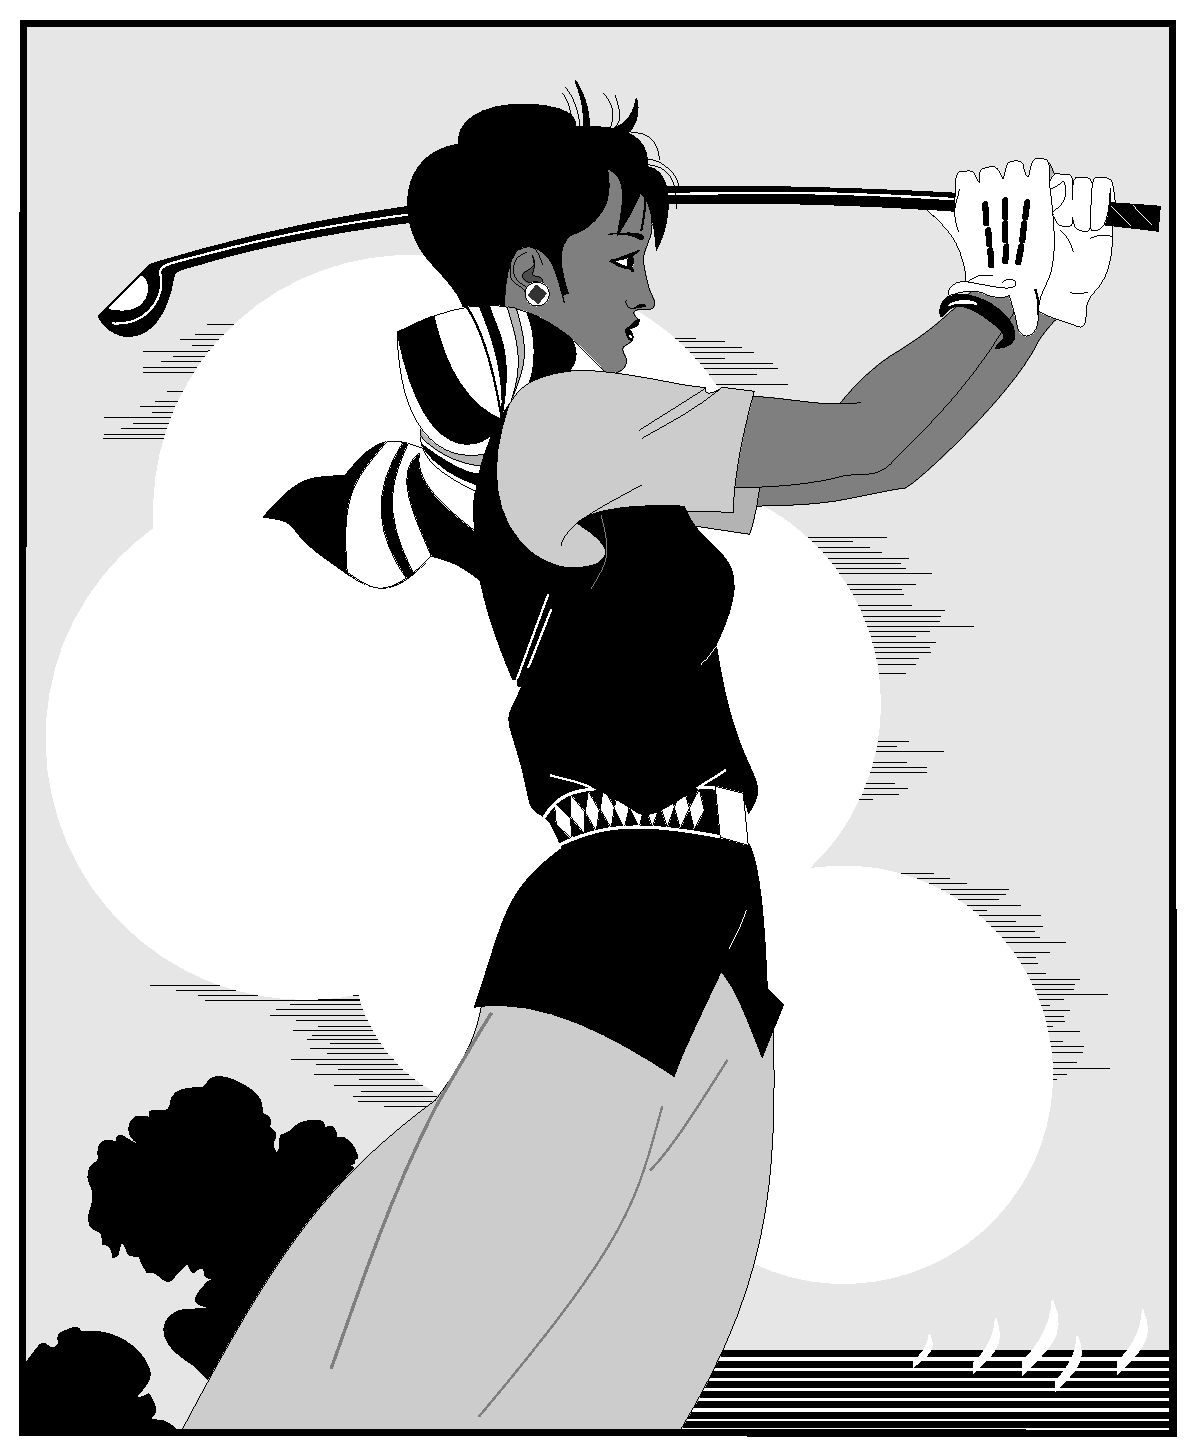
\includegraphics[width = 0.4\textwidth]{golfer}
\FigCaption{��߶�������˴�߶�������˴�߶���߶�������˴�߶�������˴�߶�������˴�߶�������˴�߶��������}
\label{Figure:Tricks:Example12}
\end{figure}
�������֣�Windows ��ֻ�Ƽ���ѵ�~CTeX ��װ����Ϊ˿������Ҫ�Լ����ã���װ��Ϳ���ʹ�á�
������У԰���û����Դ�~ \url{ftp://202.118.224.241/software/Science/TeX&LaTeX/CTex/} ����~
CTeX-2.4.5-8-Full.exe ��~ CTeX-Fonts-2.4.4.exe���Ȱ�װ��װϵͳ��Ȼ��װ���塣��У԰���û�
���Դ�~ \href{http://www.ctex.org}{CTeX�Ĺٷ���վ} �����������ļ���

\subsection{�Ƽ�����������}

������ǵ�һ�νӴ�~ LaTeX����ô��װ~ CTeX ֮�󣬲�Ҫֱ�Ӵ򿪱༭����~WinEdt ���в�������Ϊ���������������˽⻹���٣��������ʴӡ����~ Windows
ϵͳ�Ŀ�ʼ~ $\rightarrow$ ����~ $\rightarrow$ ���� TeX ��װ~ $\rightarrow$ help $\rightarrow$
�����ĵ��˰ɣ����ǽ����˳���ǣ����ȴ�~ CTeX FAQ����ͷ����''��������''��һ�ڣ�Ȼ��
��ͬһĿ¼�´�~ LShort-cn �ļ�����ͷ��β�������һ�飬���ó��Լ�ס���е����
ֻҪ�˽�~ LaTeX ���ص㣬��ÿһ������һ��������ʶ�Ϳ��ԡ��Ժ��㻹���Ի�ͷ������������
Ȼ��� ~CTeX FAQ �����ϣ�����������У����Գ���ȥ��ϰ�Ű�һЩ�ĵ����鿴����Ч��������~ WinEdt ����
�����뿴����Ľ� \ref{sec:winedttricks}����

������⵽���������ĵ�~PDF: latex2e ��ͼָ�Ϻ�~mathematics (LaTeX ���� The LaTeX Companion ��~chapter8)��
�ֱ��ǽ���ͼ֪ʶ�͹�ʽ���뷽���ģ�������ϸ������Ҳ���һ�¡����ڹ�ʽ���룬����һ���ر�ֵ���Ƽ�����
\href{http://www.tug.org/tex-archive/info/math/voss/mathmode/}{mathmode 2.0}��У԰���û������Դ�
\href{ftp://202.118.224.241/software/Science/TeX&LaTeX/TeX documents/}{У��~FTP TeX ����Ŀ¼}���ء�

\begin{figure}[htbp]
\centering
\subfigure[�߶���]{\label{Figure:Tricks:Example2:a}
  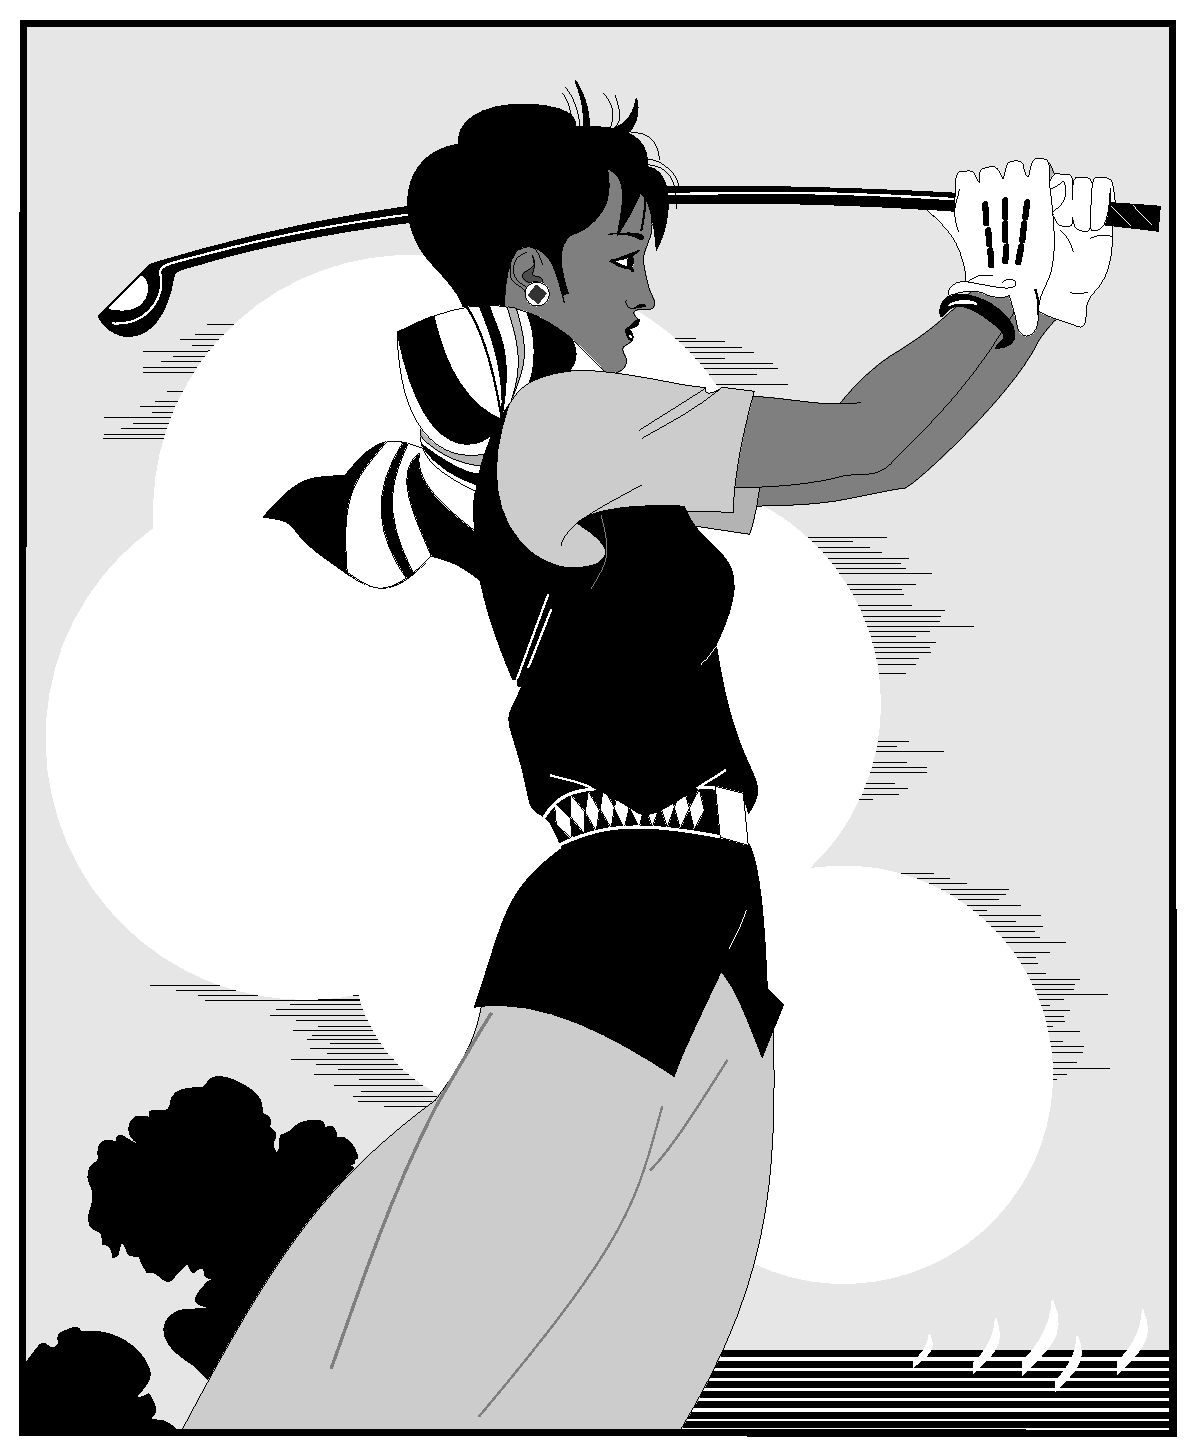
\includegraphics[width = 0.22\textwidth]{golfer}
}
\subfigure[�߶���]{\label{Figure:Tricks:Example2:B}
  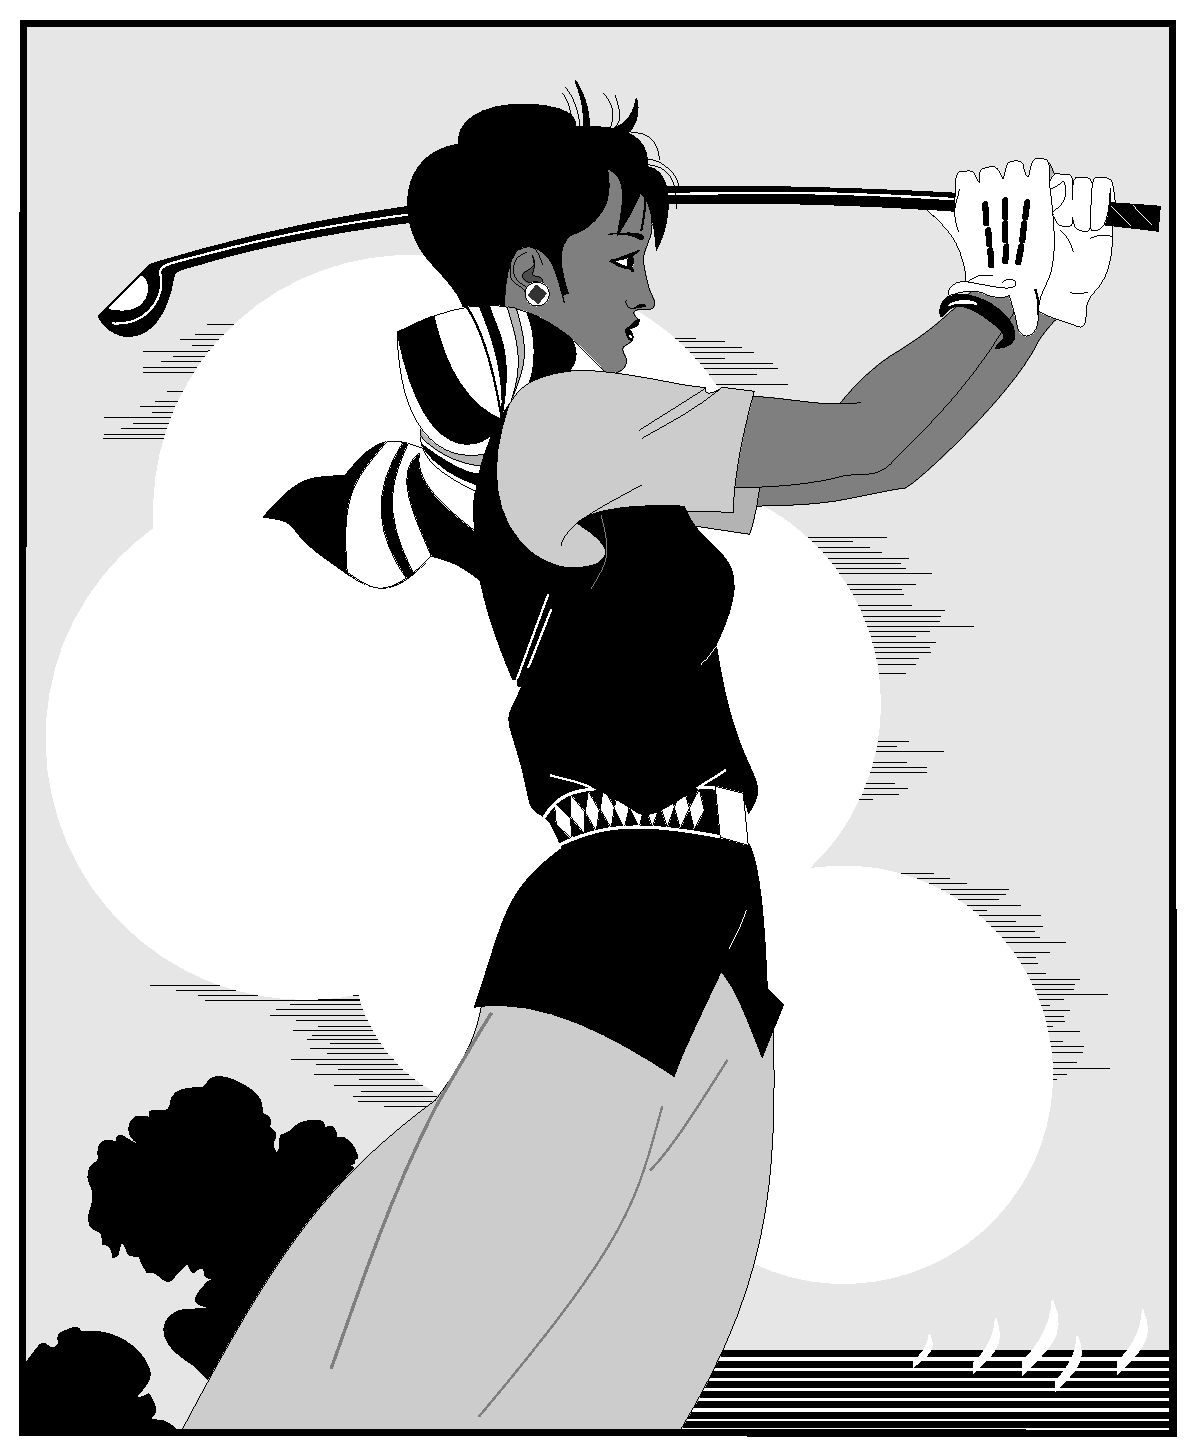
\includegraphics[width = 0.22\textwidth]{golfer}
}
\FigCaption{�߶���}
\label{Figure:Tricks:Example2}
\end{figure}

\begin{figure}[htbp]
\centering
\begin{minipage}{0.25\textwidth}
\centering
\subfigure[�߶���]{\label{Figure:Tricks:Example3:a}
  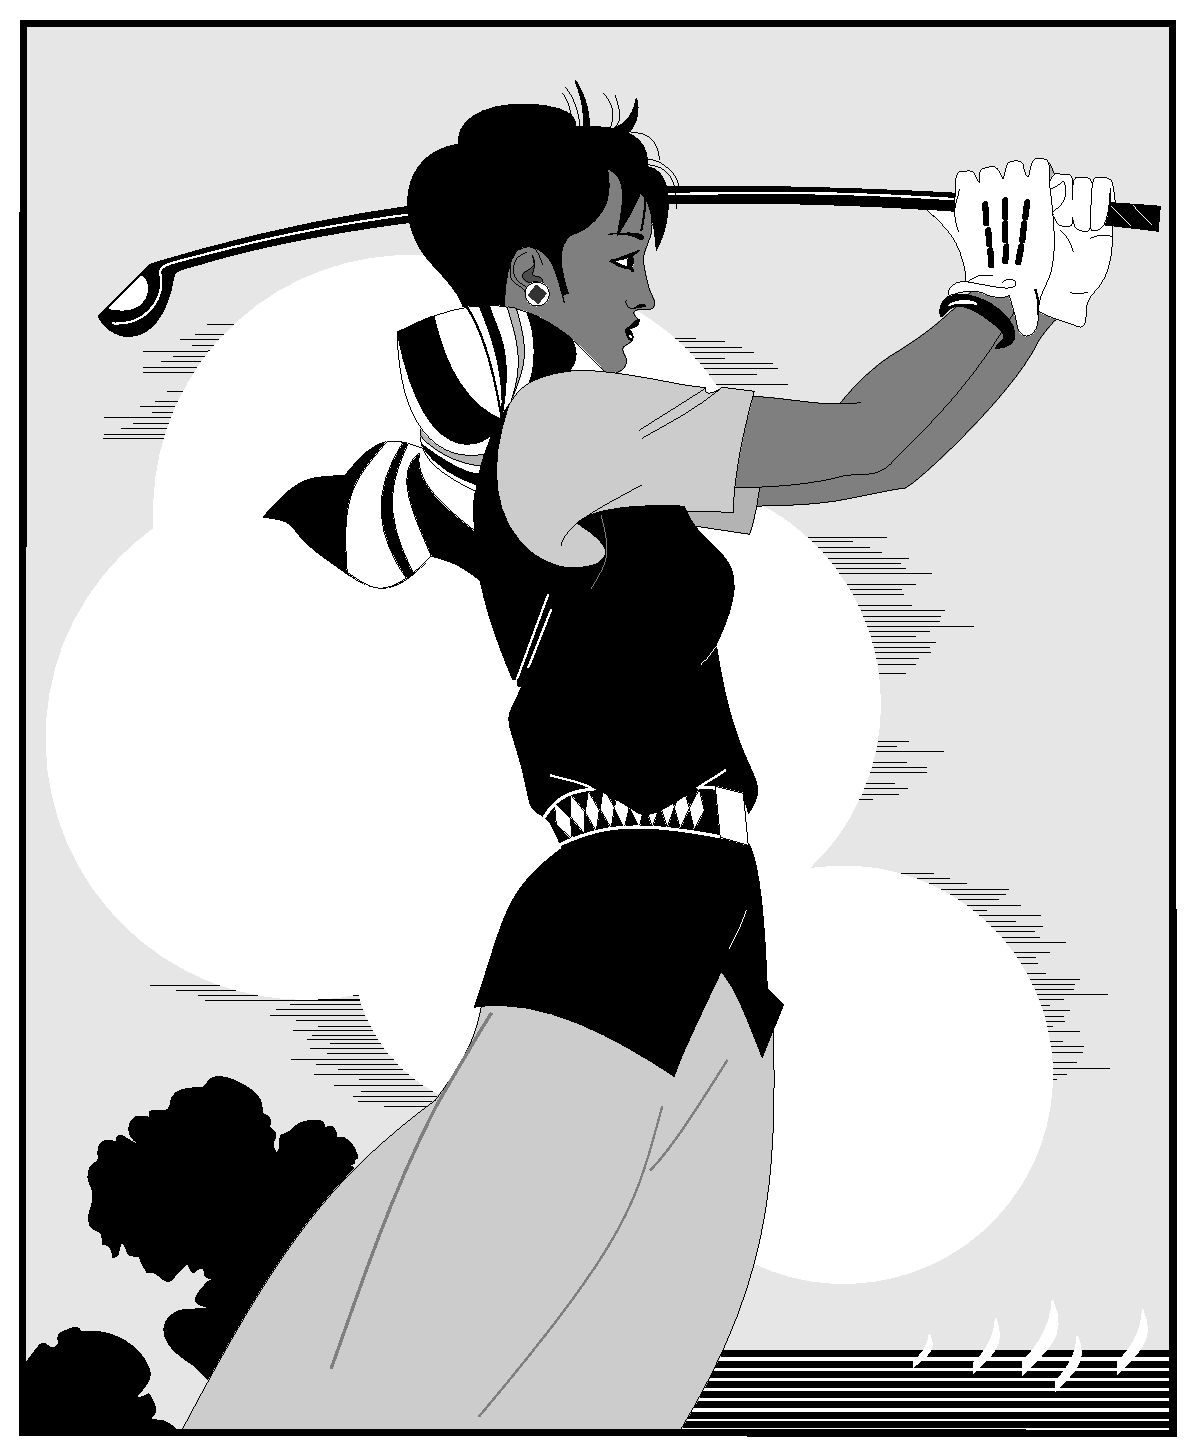
\includegraphics[width = \textwidth]{golfer}
}
\end{minipage}
\begin{minipage}{0.25\textwidth}
\centering
\subfigure[�߶���]{\label{Figure:Tricks:Example3:B}
  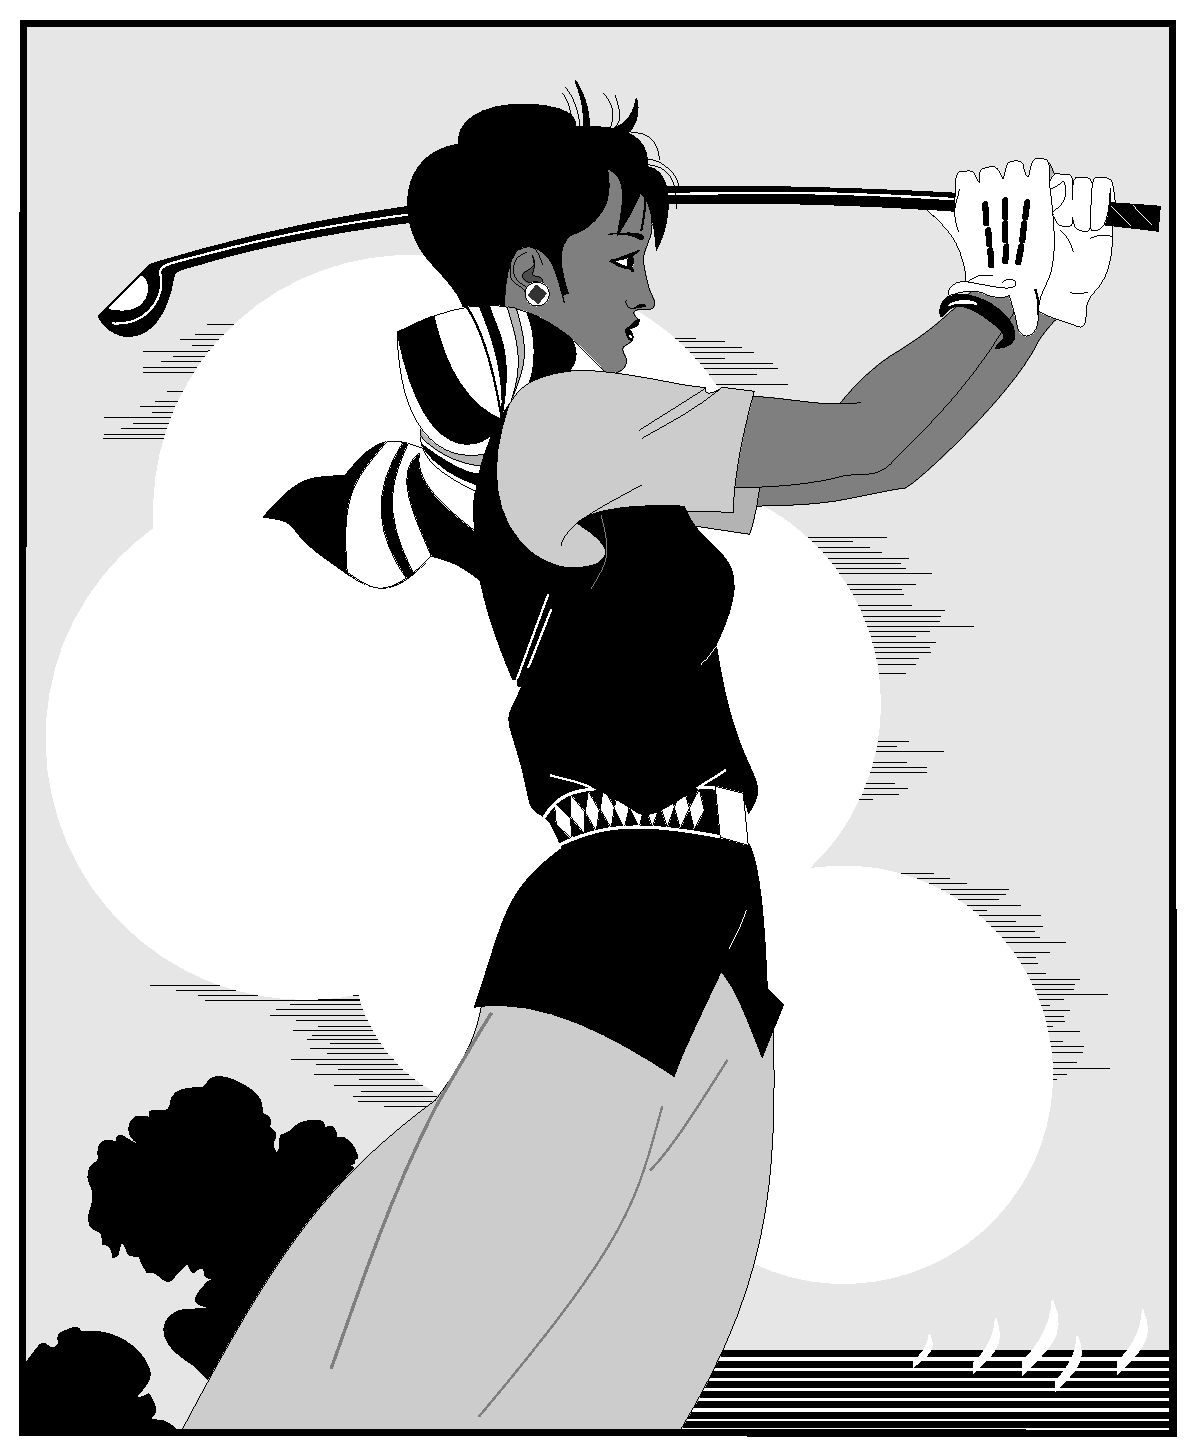
\includegraphics[width = \textwidth]{golfer}
}
\end{minipage}
\begin{minipage}{0.25\textwidth}
\centering
\subfigure[�߶���3]{\label{Figure:Tricks:Example3:C}
  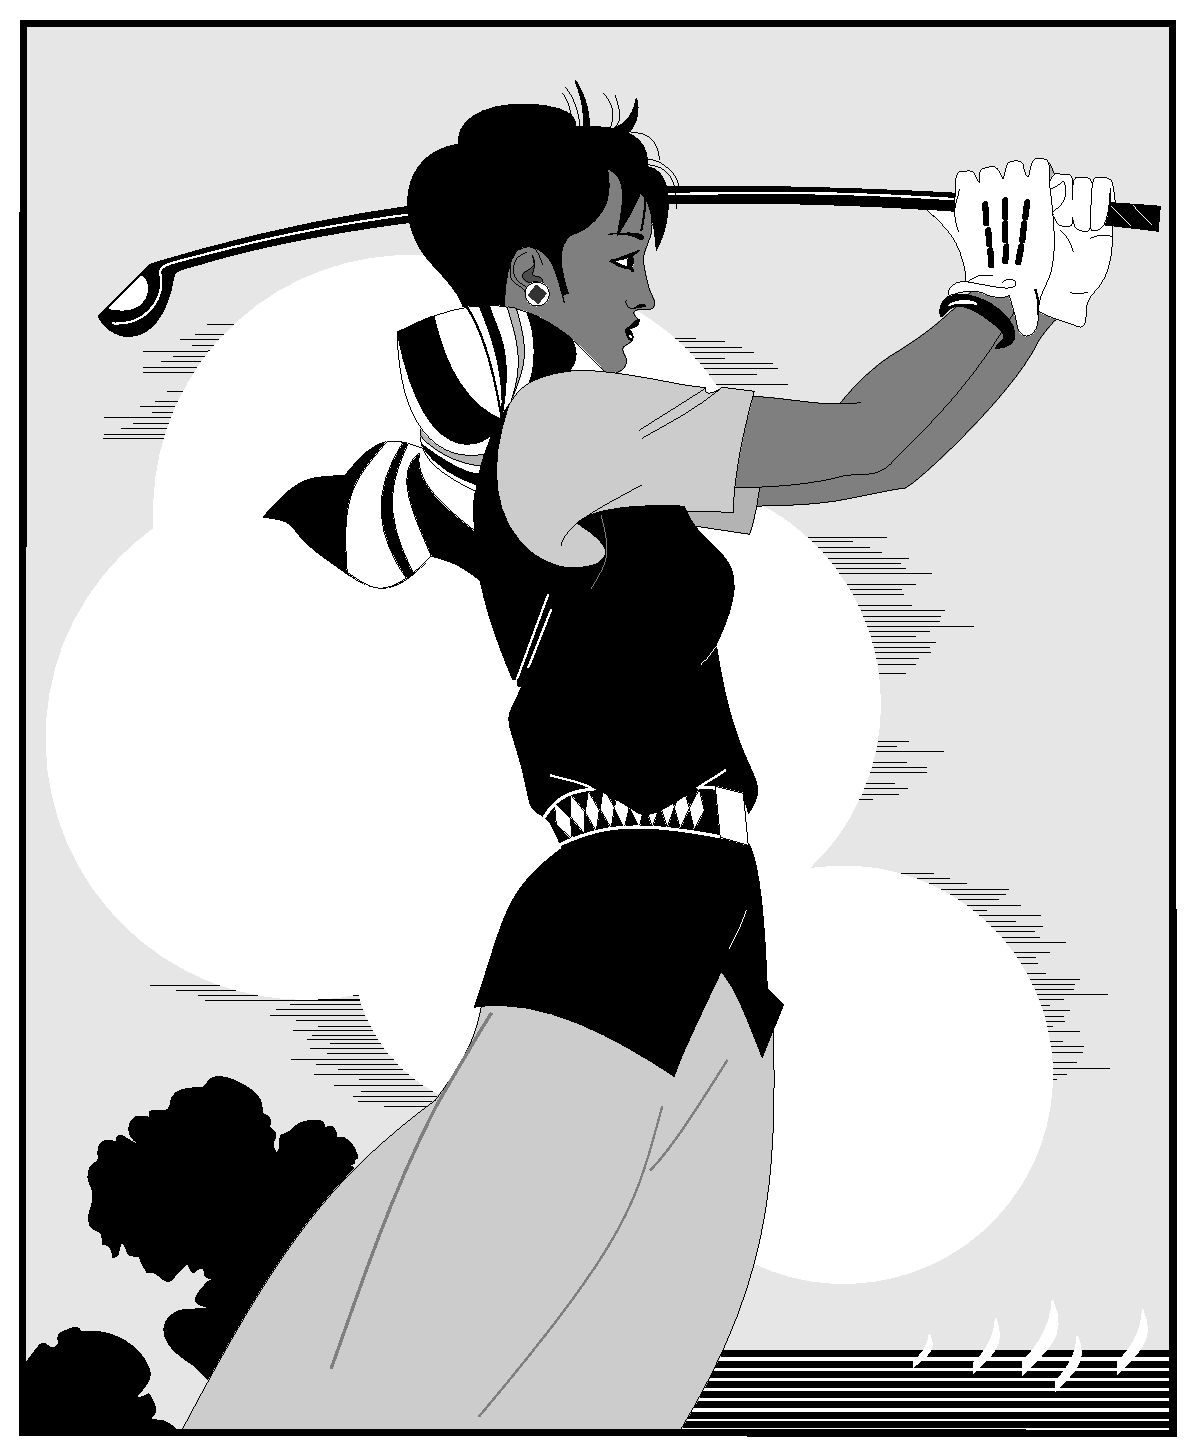
\includegraphics[width = \textwidth]{golfer}
}
\end{minipage}
\FigCaption{�߶���}
\label{Figure:Tricks:Example3}
\end{figure}

\begin{longtable}{lll}
\LTCaption{���ı����}\\
\bfseries Entity & \bfseries Unicode Name & \bfseries Unicode \\ \hline
\endfirsthead
\bfseries Entity & \bfseries Unicode Name & \bfseries Unicode \\ \hline
\endhead
\hline \multicolumn{3}{r}{\emph{Continued on next page}}
\endfoot
\hline
\endlastfoot
a&emf&bcdef\\
a&emf&bcdef\\
a&emf&bcdef\\
a&emf&bcdef\\
a&emf&bcdef\\
a&emf&bcdef\\
a&emf&bcdef\\
a&emf&bcdef\\
a&emf&bcdef\\
a&emf&bcdef\\
a&emf&bcdef\\
a&emf&bcdef\\
a&emf&bcdef\\
a&emf&bcdef\\
a&emf&bcdef\\
a&emf&bcdef\\
a&emf&bcdef\\
a&emf&bcdef\\
a&emf&bcdef\\
a&emf&bcdef\\
%a&emf&bcdef\\
\end{longtable}


\begin{table}[htbp]
\centering
\TabCaption{�������}
\label{Tricks:Tab1}
\begin{tabular}{c|c|c}
  \hline
  % after \\: \hline or \cline{col1-col2} \cline{col3-col4} ...
  ���� & ����~(\%) & �ٶ�~(ms) \\
  \hline
  С���任 & $99.8$ &  20\\
  ����Ҷ�任 & $99.0$ & 30 \\
  \hline
\end{tabular}
\end{table}

\subsection{��ʽ}
\label{Tricks:Equations}

�ı��е���ѧ���ź͹�ʽ������ķ������룺

������ѧ��������ȡ��һ���������ģ�;���ͨ����˵��$N$�����⣬����һ
�������£����о������屻�����ʵ㣬$N$��������򵥵ľ��Ƕ������⡣��һ
������ϵͳ�У�$N$��������������$n$���������$k$��С����($N=n+k$)������
$k$��С�������$n$�����������С���Ժ����˶���Ӱ�켸�����ÿ��ǣ���$k$
��С����֮��������Ͻ�������֮����໥����Ӧ�迼�ǣ���͹���������
��($n+k$)�����⡣�ر�أ���$N=3,~n=2,~k=1$ʱ����ͨ����˵���������������⡣


���������ѧ��ʽ������ŵģ�
\begin{equation}
\ddot{\mathbf{r}}=\mathbf{F}_{0}(r)+\mathbf{F}_{\varepsilon}(\mathbf{r},\dot{\mathbf{r}},t)
\end{equation}

����һ��������ŵ����ӣ�
\begin{displaymath}
F_{\varepsilon}/F_{0}=O (\varepsilon)
\end{displaymath}

\FloatBarrier %���������
���͵Ĺ�ʽ�ӷ���˵�������ӣ�

Ŀ���������׷�ٷ�����֮�������˶�����Ϊ��
\begin{equation}\label{eq:1}
\ddot{\boldsymbol{\rho}}-\frac{\mu}{R_{t}^{3}}\left( 3\mathbf{R_{t}}\frac{\mathbf{R_{t}\rho}}{R_{t}^{2}}-\boldsymbol{\rho}\right)=\mathbf{a}
\end{equation}
����

$\boldsymbol{\rho}$---׷�ٷ�������Ŀ�������֮������λ��ʸ����

$\ddot{\boldsymbol{\rho}}$---׷�ٷ�������Ŀ�������֮�����Լ��ٶȣ�

$\mathbf{a}$---�����������ļ��ٶȣ�

$\mathbf{R}_{t}$---Ŀ��������ڹ�������ϵ�е�λ��ʸ����

$\omega_{t}$---Ŀ��������Ĺ�����ٶȣ�

$\mathbf{g}=\frac{\mu}{R_{t}^{3}}\left(
3\mathbf{R_{t}}\frac{\mathbf{R_{t}\rho}}{R_{t}^{2}}-\boldsymbol{\rho}\right)=\omega_{t}^{2}\frac{R_{t}}{p}\left(
3\mathbf{R_{t}}\frac{\mathbf{R_{t}\rho}}{R_{t}^{2}}-\boldsymbol{\rho}\right)$---�������ٶȣ�����$p$��Ŀ��������Ĺ����ͨ����

��ʽ�ӷ���˵��������������
\begin{equation}\label{eq:111}
\ddot{\boldsymbol{\rho}}-\frac{\mu}{R_{t}^{3}}\left( 3\mathbf{R_{t}}\frac{\mathbf{R_{t}\rho}}{R_{t}^{2}}-\boldsymbol{\rho}\right)=\mathbf{a}
\end{equation}
\begin{formulasymb}{ʽ��}{-15pt}%-3pt,-20pt�����Ϸ��ļ�ࡣ
  \fdesfirst{$\boldsymbol{\rho}$}{׷�ٷ�������Ŀ�������֮������λ��ʸ����}
  \fdes{$\ddot{\boldsymbol{\rho}}$}{׷�ٷ�������Ŀ�������֮�����Լ��ٶȣ�}
  \fdes{$\mathbf{a}$}{�����������ļ��ٶȣ�}
  \fdes{$\mathbf{R}_{t}$}{Ŀ��������ڹ�������ϵ�е�λ��ʸ����}
  \fdes{$\omega_{t}$}{Ŀ��������Ĺ�����ٶȣ�}
  \fdes{$\mathbf{g}=\frac{\mu}{R_{t}^{3}}\left(
3\mathbf{R_{t}}\frac{\mathbf{R_{t}\rho}}{R_{t}^{2}}-\boldsymbol{\rho}\right)=\omega_{t}^{2}\frac{R_{t}}{p}\left(
3\mathbf{R_{t}}\frac{\mathbf{R_{t}\rho}}{R_{t}^{2}}-\boldsymbol{\rho}\right)$}{�������ٶȣ�����$p$��Ŀ��������Ĺ����ͨ����}
\end{formulasymb}

\subsection{WinEdt�ı��뼰��������}
\label{sec:winedttricks}
~
��һ�ĵ�~ WinEdt\_LaTeX\_guide.doc �򵥽�����~ WinEdt �ļ��ĵ��ı��뷽�������Ե��
\url{http://bbs.hit.edu.cn/bbscon.php?bid=296&id=1887&ap=719} �õ���

������ϸ���ܱ��밴ť�ĺ��壬����һ�������ر���棬
��ע������Ľ���˳����~ WinEdt ��Ĭ������˳��
\begin{hitlist}
  \item TeX: ��������ʹ��~ TeX ����д���ĵ����ǵײ�ı���ϵͳ��
  \item LaTeX: ��������ʹ��~ LaTeX ����д���ĵ�����Ŀǰ����ʹ������~ LaTeX2e �ĵ�����ϵͳ������~ dvi �ļ���
  \item cct\& LaTeX: cct �ǹ��ڵ����ֲ��о�Ա������һ��ʹ��~ LaTeX �����������ĵ��Ľӿ�ϵͳ��
  ���Ȱ�~cct ���ĵ���~.ctx ת����~.tex ��ʽ��Ȼ����ñ�׼��~ LaTeX ����������dvi�ļ���
  \item PDFLaTeX: ����������~LaTeX������һ�ֱ���ϵͳ��ֱ������~pdf �ļ���֧�ָ����~ pdf �ļ���Ч������Ӧ��Խ��Խ�㷺���������Ļõ�Ƭ��
  \item BibTeX: ��������������ο����׵����ͨ��������һ�������ο�������Ŀ���б�~ bbl �ļ����Ű�ʹ�á�
  \item Make Index: ������������ĵ���������
  \item TeXify: ���Ǽ�����������ĺϼ������Զ�����~ LaTeX����pdflatex����MakeIndex ��~ BibTeX ��������Ҫ�Ĵ���������һ��
  ��������������б��ͽ������õ�~ dvi��pdf���ļ�������~ dvi��pdf���ļ������ɹ��̡�
  \item CTeXify: �����~ CTeX ��װ����������֧�ֵ�~TeXify ��������������ĵ�~ dvi(pdf) �ĵ���
\end{hitlist}

����ʹ���ĸ����밴ť��������ĵ����ͼ������������й�ϵ����Ϊ��ͬ�ı�����������ĵ��е�Ԫ��Ҫ��һ����
���磬��������õ���~eps ͼ�Σ�Ӧ����~latex�����룬����������~pdf ͼ�Σ�Ӧ����~pdflatex �����롣
�����������ǰ����ĵ���Ӧ��Ҳ�Ѿ������ˡ�

\subsubsection{��ʾ�ĵ��ṹͼ}

WinEdt�е�~gather�����ռ��½ڱ��⣬�γ�~TOC �б�������������~word �е��ĵ��ṹͼ����
д���ĵ���ʱ��������ܷdz����ã����������ǵ�~Pluto ģ���У��Զ�����һЩ�½ڱ��⣬
��Щ�Զ������ȱʡ��~gather �Dz�ʶ��ġ�TeX@lilac �ṩ��һ�ַ�������~WinEdt.gdi�ж�����������
��Ч��ϣ����ʹ��������ܵ����ѿ����Լ������޸ģ�tools �ļ����������޸Ĺ���~WinEdt.gdi��
������Ҳ����ֱ��ʹ�ã��ŵ�~winedt Ŀ¼���滻ͬ���ļ����ɡ�

winEdt ��~ tree interfacezho ��Ҳ��~ TOC ��һ��������ͨ���޸� ~WinedtĿ¼�µ�~WinEdtEx.iniʵ�֡���~tools�ļ�����
��~WinEdtEx.ini �滻��ͬ���ļ��Ϳ��ԡ�

������Щ�Զ���������ڱ༭״̬�²�����ȱʡ����һ������������ܸ����ͺ��ˣ�TeX ͬ���ҵ����Լ�����ķ�����
��~winedt �˵�~ option/highlighting/switches �޸ģ�tools �ļ���~ Switches.dat ������
����õģ������������˵�λ��ʹ�öԻ���������~``Load from'' ��ť���ء�

\subsection{����ͼ�ij�����ʽ}

��~latex �ĵ���д�����У����õ�ͼ�θ�ʽ��~ eps ��~ pdf ��

pdf �ļ����ɣ������úܶ��������ɣ�����~adobe acrobat ��pdffactory��pdf xchange �ȡ�
�����Ƽ�~ acrobat (ע�ⲻ��~ acrobat  reader)����Ϊ����װ������һ��~ pdf ��ӡ����
�κ�һ���ĵ�������ͨ�������ӡ������~pdf �ļ�������Ҫ�Ĺ����Ƕ�~ pdf �ļ��Ķ��༭��
pdf �ļ�������~acrobat ����вü�~ (documents,crop pages...)��ȡ������ҳ�档����֧��
ֱ������Ϊ~ eps �ļ��Ĺ��ܡ����ԣ�����~acrobat �������������е�ͼ�δ������ⶼ���Խ����
���������������ҵ������

������~latex ����ͼ�����Ƚ϶࣬���е���ͼ������~visio��~ coraldraw��~ photoshop��~ gnuplot ���ɵ�ͼ
������ͨ������ķ���ת����~eps ��~pdf �ļ������⣬���кܶ�ר��Ϊ~latex ��������ͼ������
��ͨ���������ʽ����ͼ�ģ�����~metapost��~pstricks��~asymptote��~pgf/tikz �ȣ�Ҳ�м򵥵�
������ͼ���������������~Dia��~winfig��~gclc �ȡ�  ��������������Щ����������ԱȽϼ򵥣�������ͼҲ����Ư�������Ƕ�û��΢����
~visio ��������ǿ�����Զ����������������~visio ����ͼ��

���ڲ�ͼ��������ڵ����İ��ͼָ���Ѿ�����ϸ�ˣ����ﲻ�ٽ��ܣ��뷭�ĸ��顣

\subsection{���ٲ���ͼ��}

����ͼ���Ȼ����IJ��룬WinEdt �ṩ�˺������ķ�����ֻҪѡ�񹤾�����ͼƬ�ͱ���ť���Ϳ���
����һ��������ͼ���������Ҫ��ֻ�ǰ����е��ǺŻ����Լ��Ķ����Ϳ����ˡ�
WinEdt���ṩ��һ���꣬GUI ��ʽ���ͼ�IJ�����̣�ѡ����࣬Ҳ�����㡣
��ʱ�򣬸о�����Ƚϸ��ӣ���������~LaTeX д������Գ���һ�� ~xl2latex 2.0 ���~ excel
�������Ϊ~LaTeX ����ĺꡣ������~excel �����ɱ���Ȼ������һ�º꣬�������˱����~LaTeX ���롣
ģ���~edittools Ŀ¼���ṩ����һ�ļ���

\subsection{���༼�ɼ����������ĵ�}
��������ż��ɣ����Բο��϶���TeX����õ׵�����~\href{http://bbs.hit.edu.cn/bbscon.php?board=TeX&id=2038&ftype=11}{���沿�����⵼��(��Ҫ����������)}��

\section{ģ��ʹ��˵��}

��ģ����ά���е�~v0.2 �汾��Ҳ�ǵڶ������������İ汾��������~2006 ��~5 �¿����һ��~word ����
������Ŀǰû���ѷ��ֵ�������ڣ���ӡЧ����~Word ������ࡣ������ִ��������������Ľ����飬�뷴�����϶���~bbs ��~TeX �档:-)

ע�⣺��ʹ��֮ǰ���Ŀ¼�µ�~``����.txt'' �������м��㸽�ӵ�ע��ѡ��Ժ��ӵ�ģ���ʹ��˵����ȥ�ġ�

���汾��˵���ĵ�����ʱ���ϵ����û���������������������ǰ�Ӵ���~LaTeX�����źܿ�ͻ����ֵġ�:P

\section{ģ��������¼}
\subsection{v0.11 ��һ�����������İ汾}
�ڹ�������ҵ��ѧ˶��ʿѧλ����ģ�壨SVN�ֿ�汾150������1.8rc1��Ŀǰδ������1.8rc2֮�䣩�Ļ����ϣ�LaTeX@lilac
�����˹�����о���˶��ʿ���ⱨ��ģ�塣0.11 ���Ƕ�����~2006 ��~5 �¿����һ��~word ������b5ֽ�ͣ�������Ŀǰû���ѷ��ֵ�������ڣ���ӡЧ����~Word ������ࡣ

\subsection{v0.2 ��ǰ������ģ��汾}
������ģ��汾����ϵͳ�ڲ�SVN~195 �汾��Ϊ~v0.2���������������汾��ά����Ϊ~LaTeX �� luckyfox�� ���汾�ĸĶ���Ҫ�����¼������档

\subsubsection{bugs����}
\begin{hitlist}
  \item ������``�ο�����''�ĸ�ʽ��
  \item ������ͼ����ʽ�ı�ţ����±��ȥ����
  \item �������ڷ���"˵��"�ļ�࣬��ʱ�������Ҳ���������������졣��һ��~\verb|\hfill| �Զ�����һ�¡�
  \item ���������Ķ��壬�������治��ð�š�
  \item ͼ��Ӣ�ı��� ��д �� ``Fig'' ��Ϊ``Fig.''��
  \item ���� cmap ���������λ�ã���Ӧ miktex 2.5��
\end{hitlist}


\subsubsection{������ǿ}
\begin{hitlist}
  \item ��ԭ��~b5 ֽ�͵Ļ�����������~a4 ֽ�ͣ����û�ѡ���Ƽ�ʹ��~a4 ֽ�͡�a4 �汾�������ֺ��벩ʿ���Ĺ涨һ�£���о�Ȳ�ʿ����Ҫ�󣬿�������Ϊ���ⱨ�治��װ���ɡ�
  \item �ο����µ�˶ʿ������棬�ṩ��˶ʿ�����֧�֡�
  \item �����˶� winedt5.5 ���Զ��������� tree �� gather �е� toc ��֧�֡�
\end{hitlist}


\subsubsection{�ĵ�˵��}
 \begin{hitlist}
   \item ����``ģ��ʹ��˵��''һ�ڵ�λ�ã�
   \item ����ģ��������¼;
 \end{hitlist} 

%参考文献
\defaultfont
\bibliographystyle{chinesebst}
\addtolength{\bibsep}{-0.8 em} \nocite{*}
\bibliography{reference/reference}
\clearpage

\end{document}
